\documentclass{beamer}
\usetheme{Boadilla}  %Boadilla, Madrid
\usepackage[utf8]{inputenc}
%\usepackage[ansinew]{inputenc}
% \usepackage[german]{babel}  % noetig fuer Umlaute
\usepackage[english]{babel}
\usepackage{array}
\usepackage[small]{caption}
% \usepackage{wrapfig}
\usepackage{multimedia}
\usepackage{hyperref}
\usepackage{ulem}
\usepackage{color}
\usepackage{siunitx}
\usepackage{amssymb}
\beamertemplatenavigationsymbolsempty
\usepackage{multirow}
% \usepackage{dsfont} % for identity matrix \mathds{1}
%\newcommand{\RM}[1]{\MakeUppercase{\romannumeral #1{.}}}

%%% for Code Snipplets
\usepackage{listings}
\usepackage{color}

\definecolor{dkgreen}{rgb}{0,0.6,0}
\definecolor{gray}{rgb}{0.5,0.5,0.5}
\definecolor{mauve}{rgb}{0.58,0,0.82}

\lstset{
  language=[90]Fortran,
  aboveskip=3mm,
  belowskip=3mm,
  showstringspaces=false,
  columns=fullflexible,
  basicstyle={\small\ttfamily},
  numbers=none,
  numberstyle=\small\color{gray},
  keywordstyle=\color{mauve},
  commentstyle=\color{dkgreen},
  stringstyle=\color{blue},
  breaklines=true,
  breakatwhitespace=false,
  tabsize=3
}

\usepackage{verbatim}
%---------------------------------------------------------------------

%% how to include graphics
% \begin{figure}[H]
%   \centering
%   \includegraphics[width=1\textwidth]{}
%   \caption{}
%   \label{fig:...}
% \end{figure}

%---------------------------------------------------------------------
%---------------------------------------------------------------------
%---------------------------------------------------------------------

\title{grav\_project}

\author{P. Denzel and S. Vossoughi}
\date{\today}
% \institute{Universität Zürich}
 
\begin{document}
\begin{frame}
 \LARGE
 \sf 	   grav\_project \\ 
	   Computational Science II \\

\rule{0.8\textwidth}{0.5pt} \\ % horizontal line of variable length and width
 \Large Denzel, Philipp and Vossoughi, Sara \\
\rule{0.8\textwidth}{0.5pt} \\  % horizontal line of variable length and width
  \text{Email:} \\ phdenzel@hispeed.ch; sara.vossoughi@gmail.com \\
\end{frame}
%---------------------------------------------------------------------
\begin{frame}
 \frametitle{Main assignment}
 \begin{itemize}
  \item test of a new algorithm
  \item gravitational force/acceleration
  \begin{equation*}
   \overrightarrow{a_{G}}(r,\theta) = \int_{r'}\int_{\theta'} \frac{-\sigma(r',\theta')r'dr'd\theta'}{(r^{2}+r'^{2}-2rr'\cos{(\theta-\theta')})^{\frac{3}{2}}} \left(
    \begin{array}{c}
      r-r'\cos{(\theta-\theta')} \\
      r'\sin{(\theta-\theta')}
    \end{array}
  \right)
  \end{equation*}
  \item things to be learned:
  \begin{itemize}
   \item Fortran
   \item General programming experience
   \item Code optimization
   \item Balancing speed vs. accuracy
  \end{itemize}
  \item issues:
  \begin{itemize}
   \item Time
   \item Boundary conditions
   \item Numerical stability
  \end{itemize}
 \end{itemize}
\end{frame}
%---------------------------------------------------------------------
\begin{frame}
  \frametitle{First Program}
  \begin{itemize}
   \item most accurate calculation on level 0 as a reference
   \begin{itemize}
    \item Open files
    \item Read data into arrays
    \item Loop through all grid points (i,j) (force)
    \item Nested loop through all grid centres (i',j') (density)
    \item Calculate formula inside inner loop
    \item Write force into new file
   \end{itemize}
   \item other versions (higher levels) have similar structure
  \end{itemize}
\end{frame} 
%---------------------------------------------------------------------
%%% this slide may be skipped (not that important)
% \begin{frame}[fragile]
%   \frametitle{Read Files}
%   \begin{lstlisting}
%    open(unit=8, file='/path/to/r_project.data', status='old', action='read')
%    ! read radii into 1-D array
%     do i = 1, N_r
%         read(8, '(e20.10)') r_i
%         r(i) = r_i
%     end do
%     close(unit=8)
%   \end{lstlisting}
%   for $r(N\_r)$, $theta(N\_theta)$, $sigma(N\_r,N\_theta)$, $dr(N\_r)$ and $dtheta(N\_theta)$
% \end{frame}
%---------------------------------------------------------------------
\begin{frame}[fragile]
  \frametitle{Simple Implementation}
  \lstset{
    language=[90]Fortran,
    aboveskip=3mm,
    belowskip=3mm,
    showstringspaces=false,
    columns=fullflexible,
    basicstyle={\tiny\ttfamily},
    numbers=none,
    numberstyle=\small\color{gray},
    keywordstyle=\color{mauve},
    commentstyle=\color{dkgreen},
    stringstyle=\color{blue},
    breaklines=true,
    breakatwhitespace=false,
    tabsize=3
}
      
  \begin{lstlisting}
  
    ! write force components for every corner in grid
    do i = 1, N_r
        r_i = r(i)-.5*dr(i) ! shift r to the corners
        do j = 1, N_theta
            theta_j = theta(j)-.5*dtheta(j) ! shift theta to the corners
            ! sum up the forces onto the point (i, j)
            do iprime = 1, N_r
                do jprime = 1, N_theta
                    force_point = -sigma(iprime,jprime)*r(iprime)*dr(iprime)*dtheta(jprime)/(r_i**2+r(iprime)**2-2.*r_i*r(iprime)*cos(theta_j-theta(jprime)))**(1.5)
                    f_r = f_r + force_point * (r_i-r(iprime)*cos(theta_j-theta(jprime)))
                    f_theta = f_theta + force_point * r(iprime)*sin(theta_j-theta(jprime))
                end do
            end do
        write(11, '(e20.10)') f_r
        write(12, '(e20.10)') f_theta
        f_r = 0.
        f_theta = 0.
        end do
    end do
  \end{lstlisting}
\end{frame}
%---------------------------------------------------------------------
\begin{frame}
 \frametitle{Optimization Strategies}
 \begin{itemize}
  \item Fortran loops are column-major (todo:arrays?)
  \item minimizing loop overhead:
  \begin{itemize}
   \item Avoid subroutine calls in inner loops
   \item Reduce repeat evalutions by shifting to outer loops
  \end{itemize}
  \item Loop unrolling (if compiler optimization doesn't already do it)
  \item Faster arithmetic operations, e.g. a\textasteriskcentered a instead of a\textasteriskcentered\textasteriskcentered2 (multiplications instead of exponentials and logarithms)
  \item Idea: find faster methods, e.g. invsqrt using bit shifts and Newton iterations (additions and multiplications instead of divisions)
  \item Precalculations of lookup tables for grid given parameters ($cos$, $sin$, $r\_prime$, $theta\_prime$ etc.)
  \item Using symmetries
 
 \item[] $\longrightarrow$ time optimization from 255.95s to 9.87 s (v. 1)
 \item[] $\longrightarrow$ time optimization from 69.0s to 11.8 s (v. 2)
\end{itemize}
\end{frame}
%---------------------------------------------------------------------
\begin{frame}
 \frametitle{Density map}
 \begin{figure}[H]
  \centering
  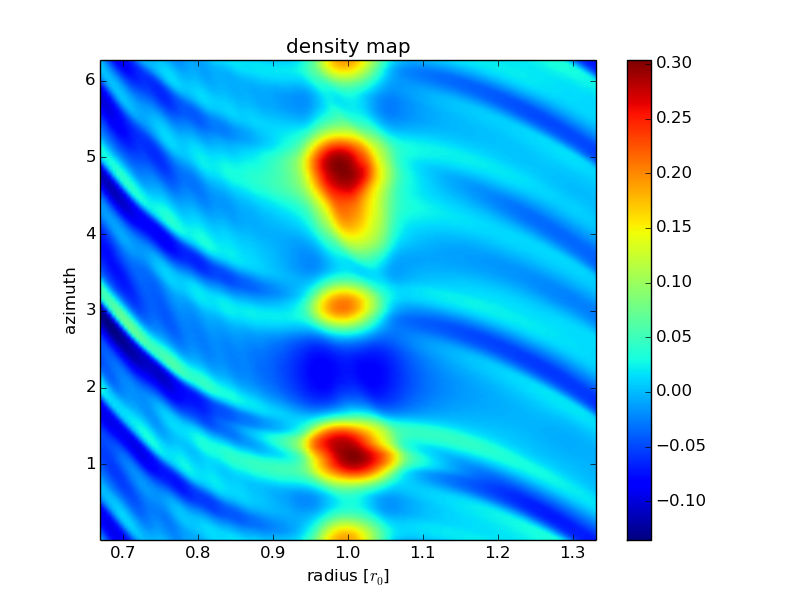
\includegraphics[width=.8\textwidth]{density.png}
 \end{figure} 
\end{frame}
%---------------------------------------------------------------------
\begin{frame}
 \frametitle{Level 0}
 \begin{figure}[H]
  \centering
  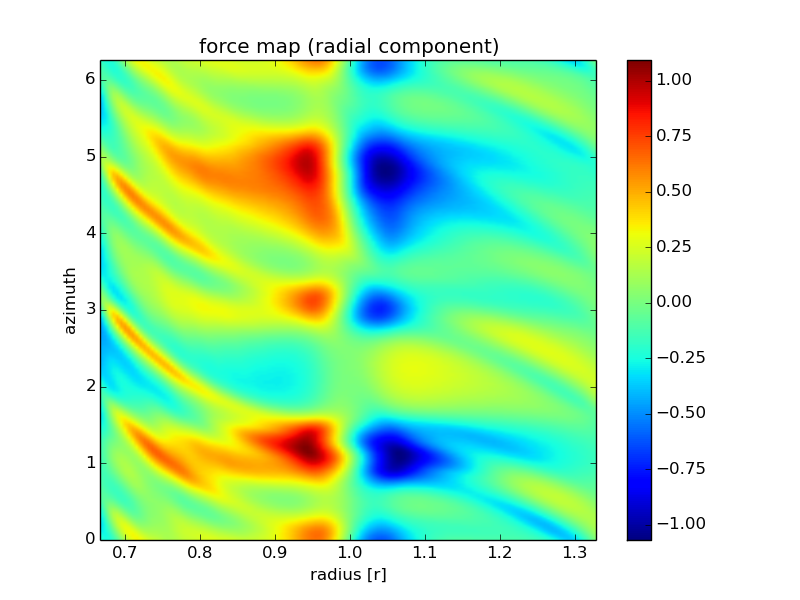
\includegraphics[width=.5\textwidth]{radial_force.png} 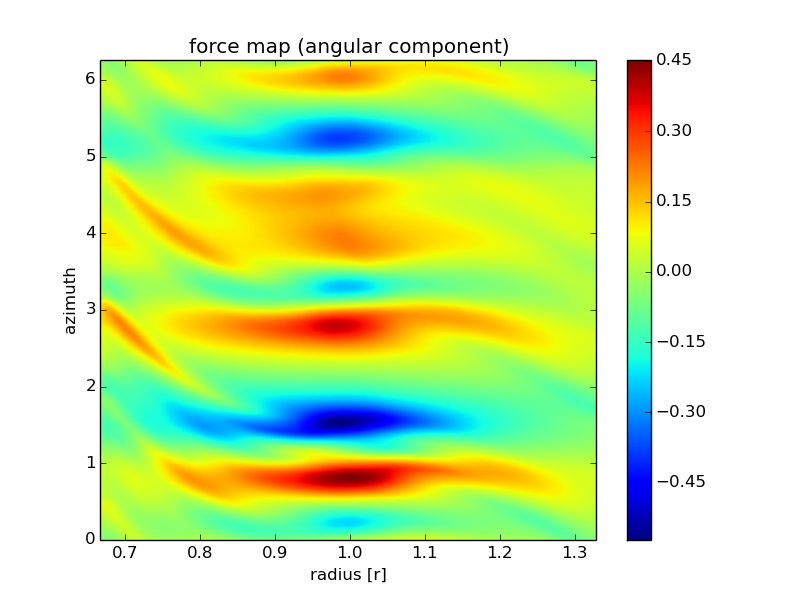
\includegraphics[width=.5\textwidth]{angular_force.png}
 \end{figure} 
\end{frame}
%---------------------------------------------------------------------
\begin{frame}
 \frametitle{Higher levels}
 \begin{itemize}
  \item Reducing operations by using fewer mass points 
  \item $4^{LEVEL}$ cells into 1
  \item Problem: oscillations
  \item Cause: calculation not anymore only at corners of the grid cells
  \item First solution:
  \begin{itemize}
   \item shift to corner
   \item interpolate the masses
   \item introduce ghost cells
  \end{itemize}
 \end{itemize}
 \begin{figure}[H]
  \centering
  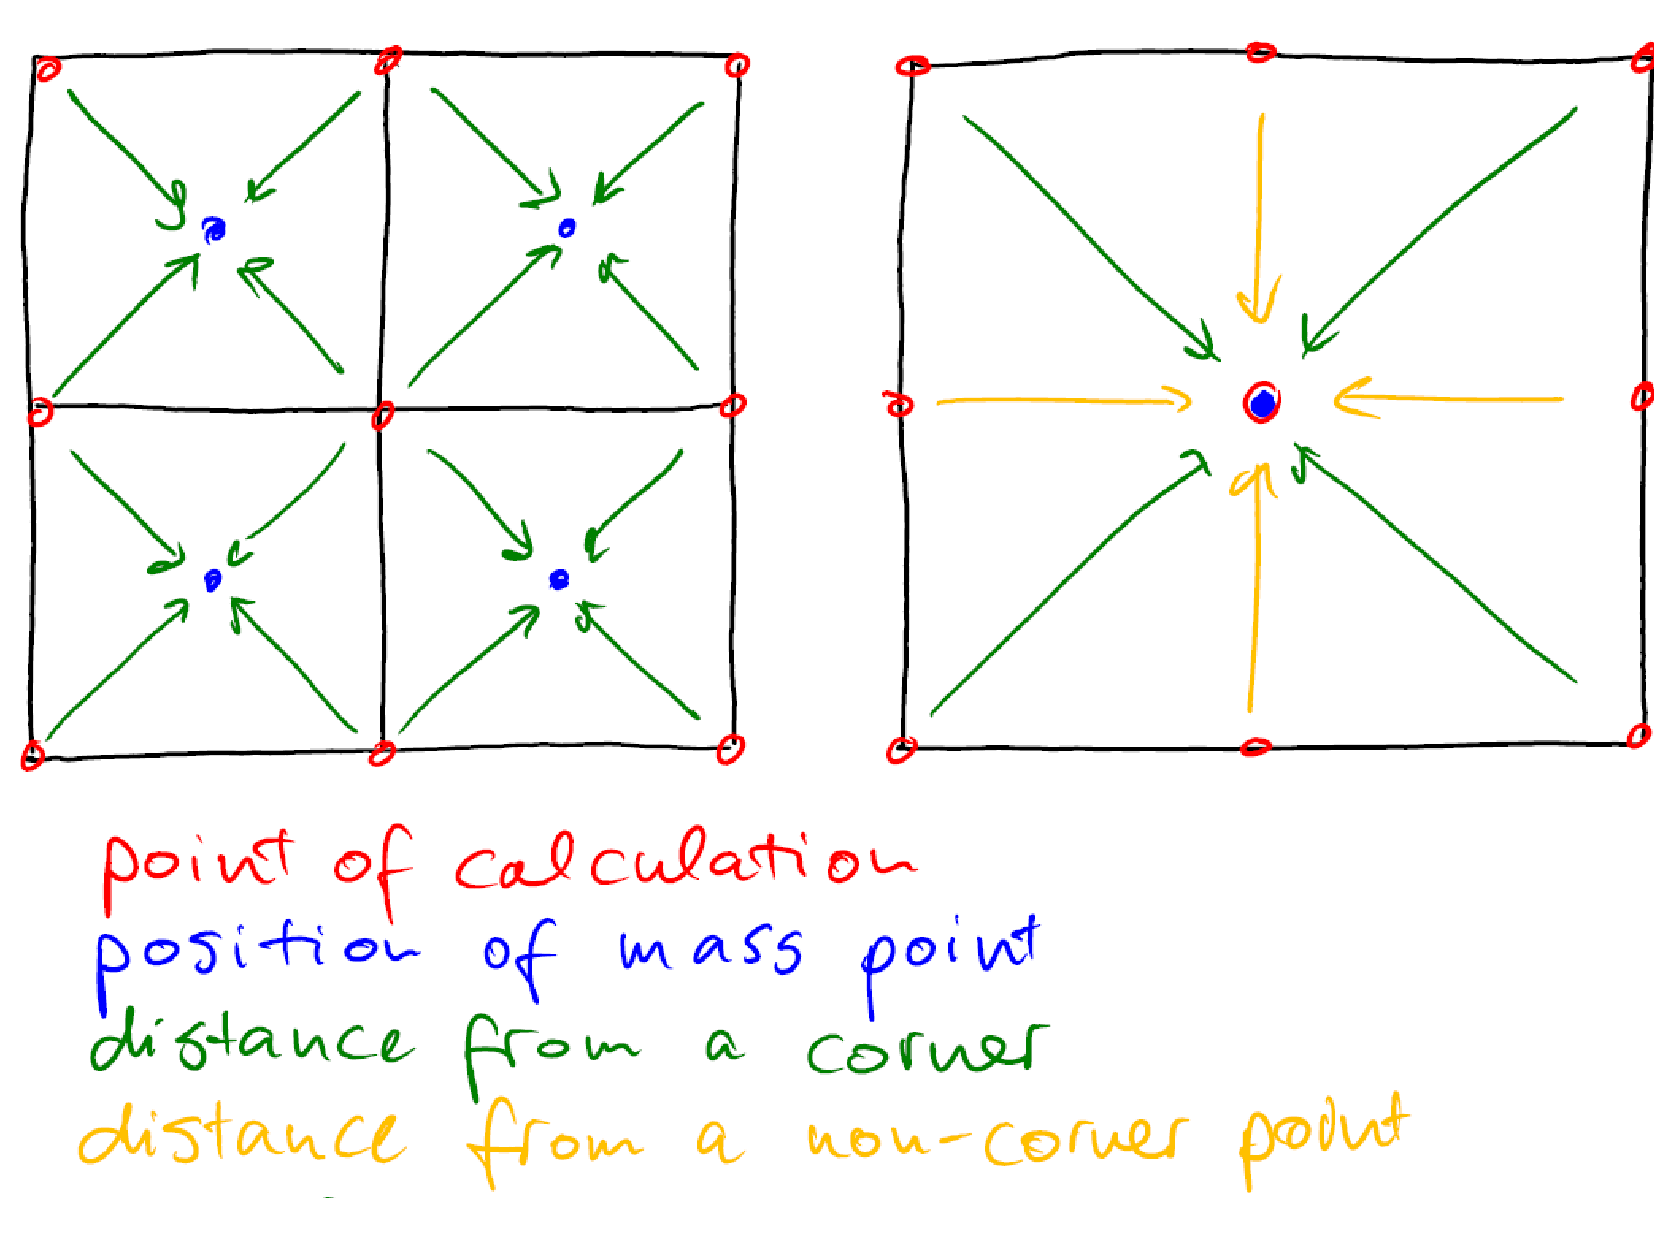
\includegraphics[width=.49\textwidth]{reimagined_sketch1.pdf}
  \caption{sketch by Philipp Denzel}
\end{figure}
\end{frame}
%---------------------------------------------------------------------
\begin{frame}
 \frametitle{Oscillation pattern (TODO: Level 3?)}
 \begin{figure}[H]
  \centering
  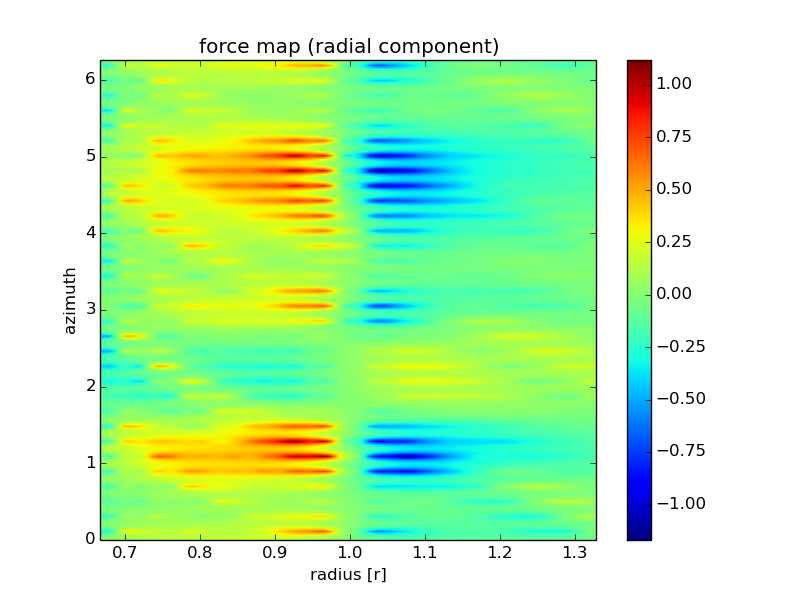
\includegraphics[width=.8\textwidth]{radial_force_lvl3.png}
 \end{figure} 
\end{frame}
%---------------------------------------------------------------------
\begin{frame}
 \frametitle{Bilinear interpolation}
 for unit square:
 \begin{equation*}
  f(x,y) \approx f(0,0)(1-x)(1-y) + f(1,0)x(1-y) + f(0,1)(1-x)y + f(1,1)xy
 \end{equation*}
 \begin{equation*}
 f(\alpha,\beta) \approx f(0,0)(1-\alpha)(1-\beta) + f(1,0)\alpha(1-\beta) + f(0,1)(1-\alpha)\beta + f(1,1)\alpha\beta
  \end{equation*}

 \begin{figure}[H]
  \centering
  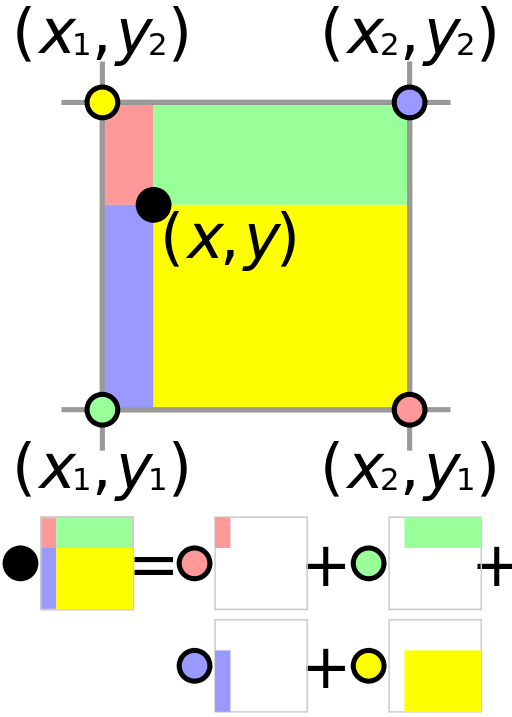
\includegraphics[width=0.3\textwidth]{bilinear_interpolation_visualisation.png}
  \caption{http://upload.wikimedia.org/wikipedia/commons/9/91/7
	   Bilinear\_interpolation\_visualisation.svg} % source link isn't getting smaller -> on two lines
\end{figure}
\end{frame}
%---------------------------------------------------------------------
\begin{frame}
 \frametitle{Pure Levels 1, 2 and 3}
 \begin{figure}[H]
  \centering
  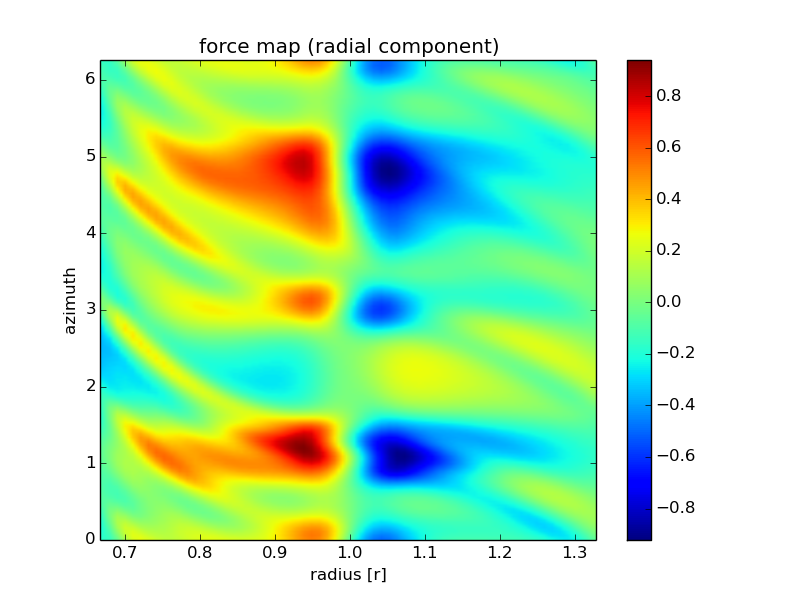
\includegraphics[width=.3\textwidth]{radial_pure_lvl1.png} 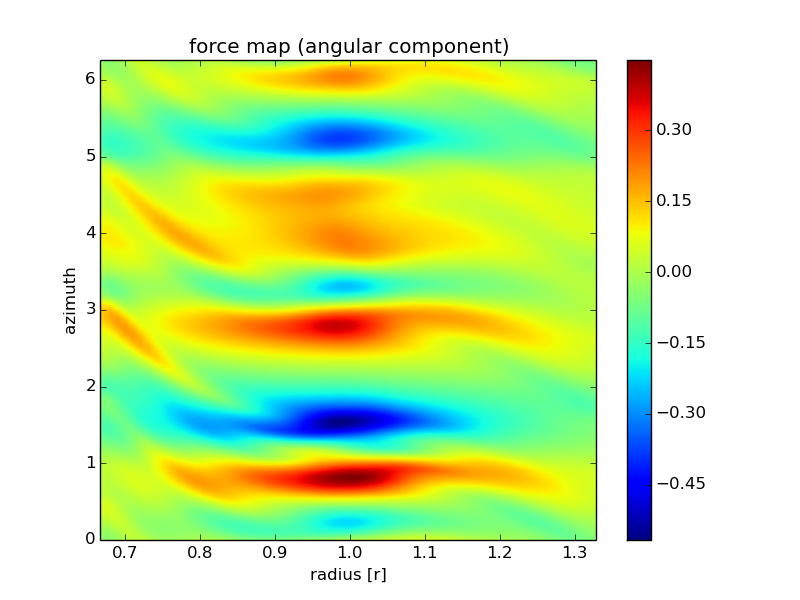
\includegraphics[width=.3\textwidth]{angular_pure_lvl1.png} \\
  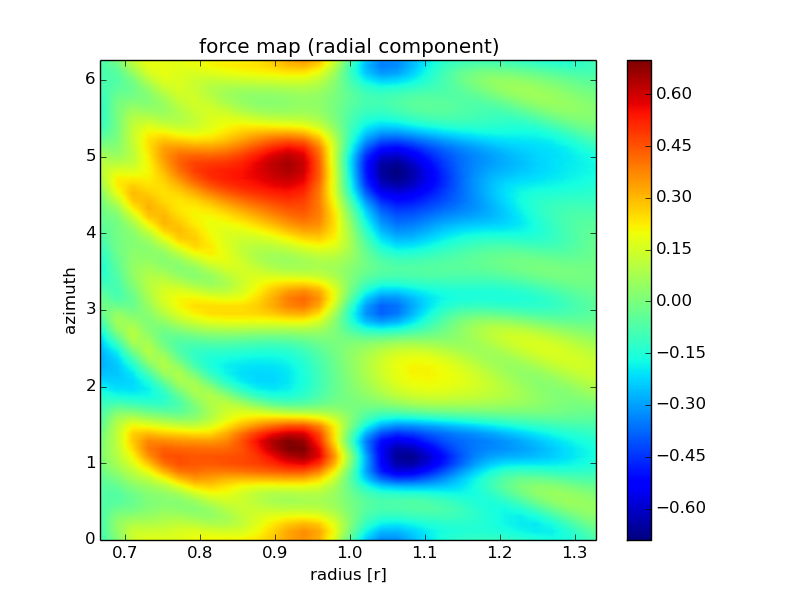
\includegraphics[width=.3\textwidth]{radial_pure_lvl2.png} 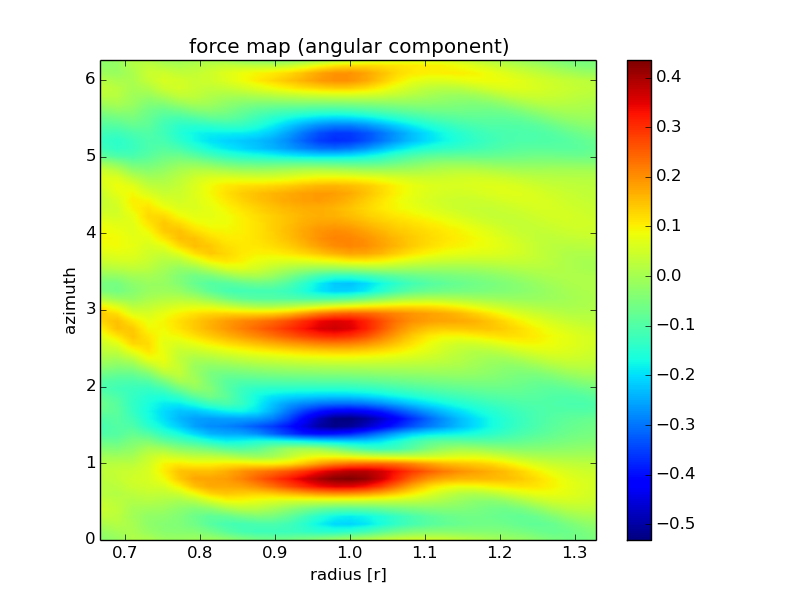
\includegraphics[width=.3\textwidth]{angular_pure_lvl2.png} \\
  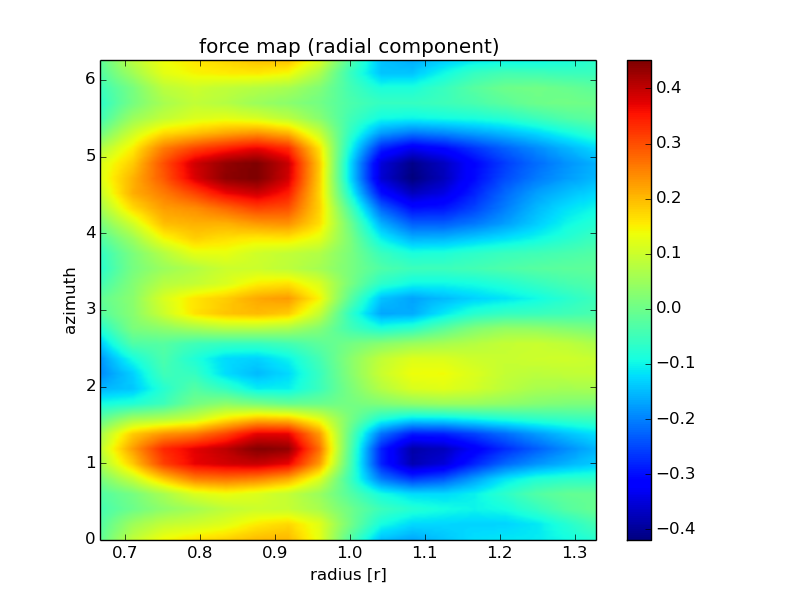
\includegraphics[width=.3\textwidth]{radial_pure_lvl3.png} 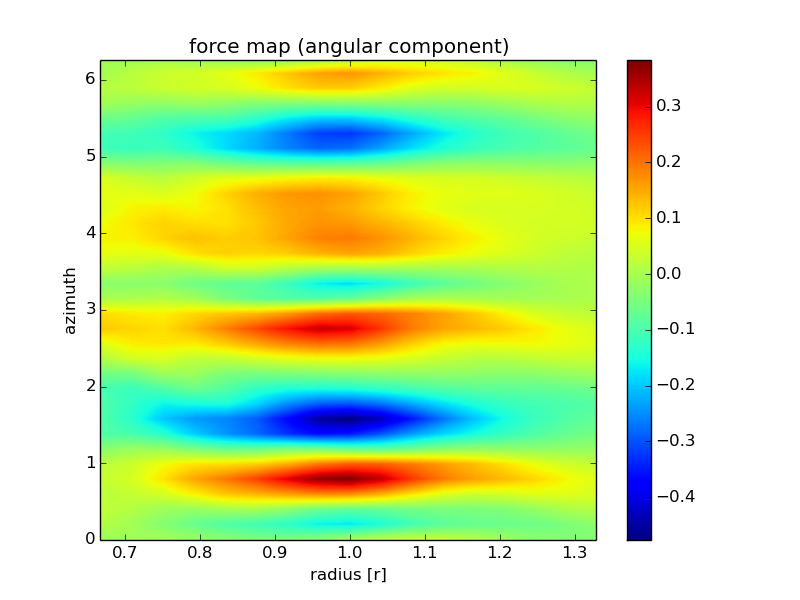
\includegraphics[width=.3\textwidth]{angular_pure_lvl3.png} 
 \end{figure} 
\end{frame}
%---------------------------------------------------------------------
\begin{frame}
 \frametitle{Refinement with a single level}
 \begin{itemize}
  \item task: calculate level 3 grid with refinement from level 2
  \item closest 4 by 4 cells calculated with one level below
  \item problem: periodic boundary conditions
 \end{itemize}
 \begin{figure}[H]
  \centering
  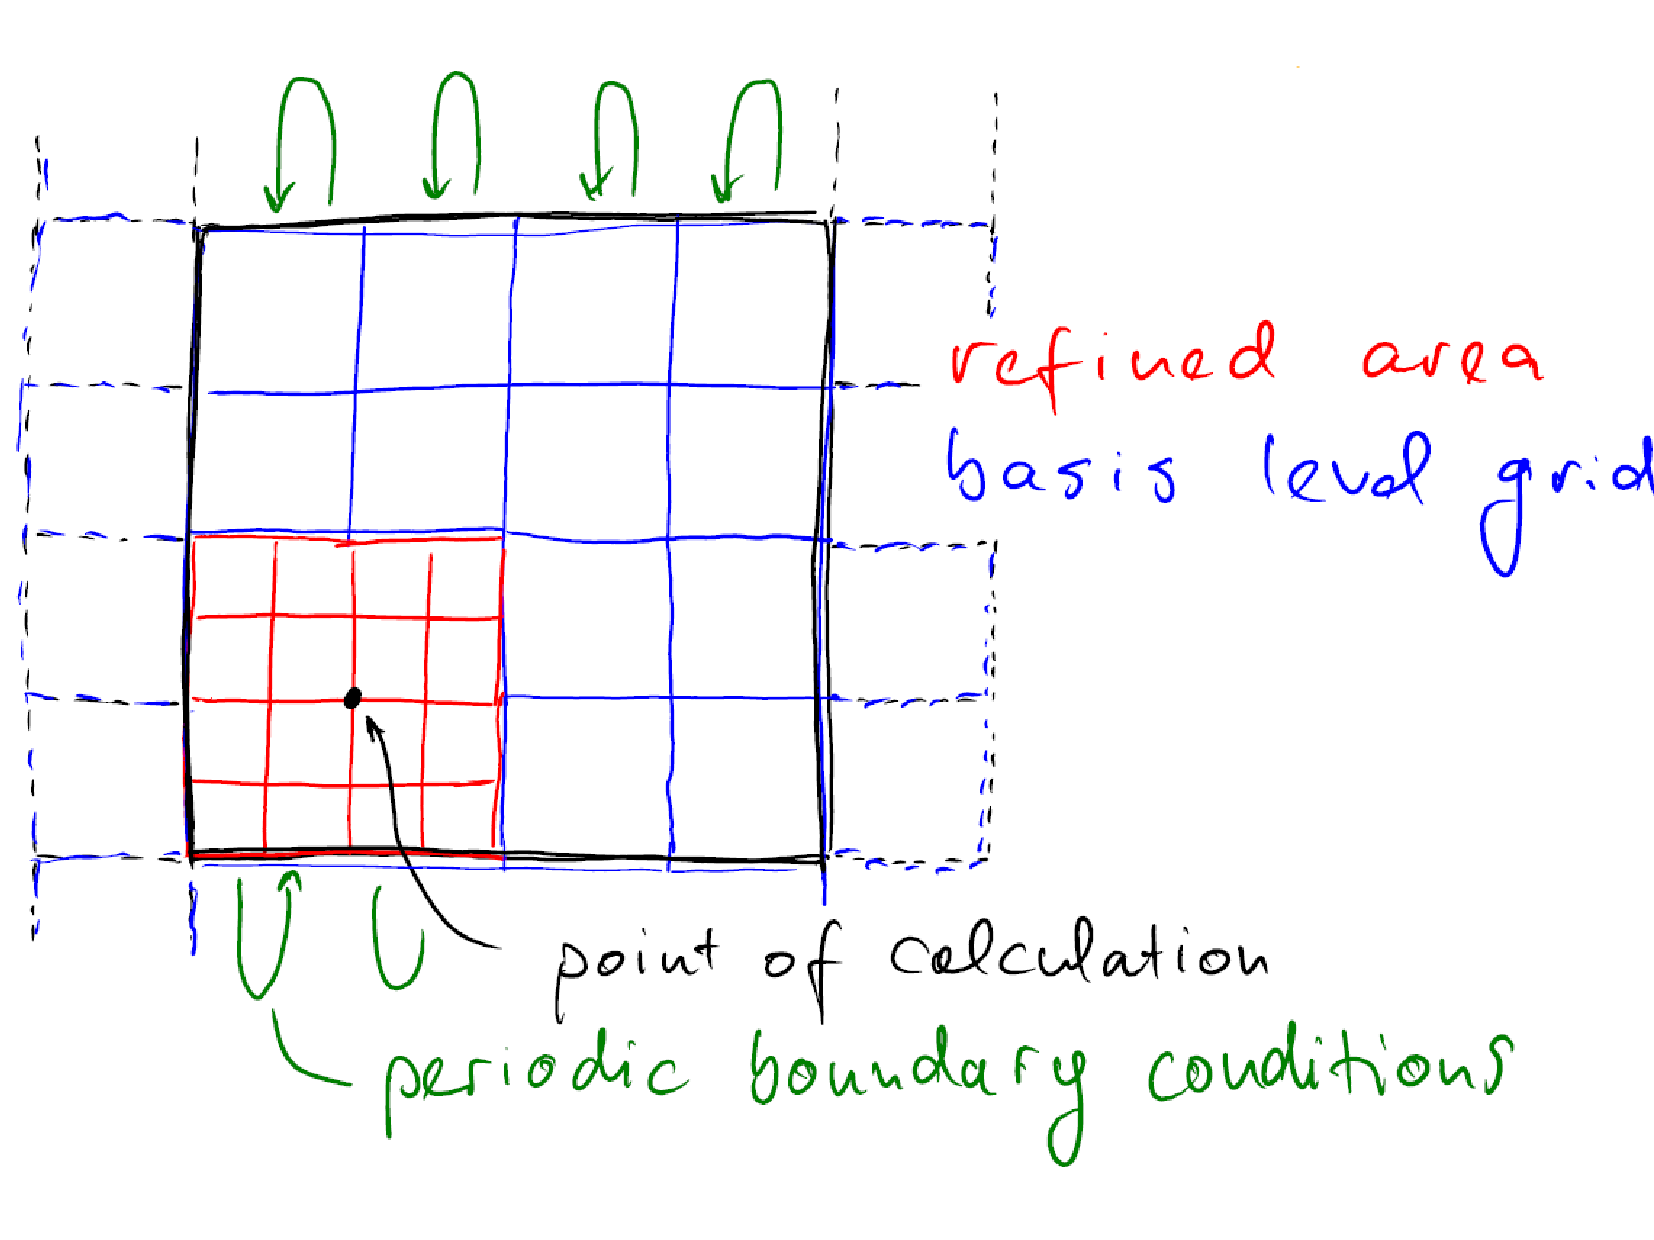
\includegraphics[width=.5\textwidth]{reimagined_sketch2.pdf}
  \caption{sketch by Philipp Denzel}
\end{figure}
\end{frame}
%---------------------------------------------------------------------
\begin{frame}[fragile]
 \frametitle{Code}
 \lstset{
    language=[90]Fortran,
    aboveskip=3mm,
    belowskip=3mm,
    showstringspaces=false,
    columns=fullflexible,
    basicstyle={\tiny\ttfamily},
    numbers=none,
    numberstyle=\small\color{gray},
    keywordstyle=\color{mauve},
    commentstyle=\color{dkgreen},
    stringstyle=\color{blue},
    breaklines=true,
    breakatwhitespace=false,
    tabsize=3
}
 \begin{lstlisting}
  do i = 1, N_r0
     r_corner = r0(i)-.5*dr0(i)
     do j = 1, N_theta0
        theta_corner = theta0(j)-.5*dtheta0(j)
        call shift_param   ! gives shifts: ishift(ref), jshift(ref), dr_shift(ref), dtheta_shift(ref)
        call ref_area   ! gives refined area boundaries: iref_low/up, ix_low/up, periodic_low/up
        call intrpltn_coeff   ! gives coefficients: c1, c2, c3, c4, c1ref, c2ref, c3ref, c4ref
        do iprime = iref_low, iref_up
           do jprime = jref_low, jref_up
           ...end do
        end do
        do iprime = 0, ix_low-1
           do jprime = 1, N_thetax
           ...end do
        end do
        do iprime = ix_up+1, N_rx
           do jprime = 1, N_thetax
           ...end do
        end do
        do iprime = ix_low, ix_up
           do jprime = 1+periodic_up, jx_low-1
           ...end do
        end do
        do iprime = ix_low, ix_up
           do jprime = jx_up+1, N_thetax-periodic_low
           ...end do
        end do
     end do
  end do
 \end{lstlisting}
\end{frame}
%---------------------------------------------------------------------
\begin{frame}[fragile]
 \frametitle{Inner loop calculation}
 \lstset{
    language=[90]Fortran,
    aboveskip=3mm,
    belowskip=3mm,
    showstringspaces=false,
    columns=fullflexible,
    basicstyle={\tiny\ttfamily},
    numbers=none,
    numberstyle=\small\color{gray},
    keywordstyle=\color{mauve},
    commentstyle=\color{dkgreen},
    stringstyle=\color{blue},
    breaklines=true,
    breakatwhitespace=false,
    tabsize=3
}
 \begin{lstlisting}
  vmass = ( c1 * massx(iprime, jprime)    + c2 * massx(iprime+1, jprime)  +&
            &c3 * massx(iprime, jprime+1)+ c4 * massx(iprime+1, jprime+1))&
            & * inv_factor2
  ! calculate shifted values
  rprime = rx(iprime)+dr_shift
  ratio = r_corner/rprime
  delta_theta = theta_corner-thetax(jprime)-dtheta_shift
  cosine = cos(delta_theta)
  denom_point = 1.+ratio*ratio-2.*ratio*cosine
  denom_point = sqrt(denom_point)*denom_point*rprime*rprime
  force_point = vmass/denom_point
  force_r(i,j) = force_r(i,j)+force_point*(ratio-cosine)
  force_theta(i,j) = force_theta(i,j)+force_point*sin(delta_theta)
 \end{lstlisting}
 or for the refined area...
 \begin{lstlisting}
  vmass = ( c1ref * massxref(iprime, jprime)   + c2ref * massxref(iprime+1, jprime)  +&
            &c3ref * massx(iprime, jprime+1) + c4ref * massxref(iprime+1, jprime+1))&
            & * inv_factor2ref
  ! calculate shifted values
  rprime = rxref(iprime)+dr_shiftref
  ratio = r_corner/rprime
  delta_theta = theta_corner-thetaxref(jprime)-dtheta_shiftref
  cosine = cos(delta_theta)
  denom_point = 1.+ratio*ratio-2.*ratio*cosine
  denom_point = sqrt(denom_point)*denom_point*rprime*rprime
  force_point = vmass/denom_point
  force_r(i,j) = force_r(i,j)+force_point*(ratio-cosine)
  force_theta(i,j) = force_theta(i,j)+force_point*sin(delta_theta)
 \end{lstlisting}
\end{frame}
%---------------------------------------------------------------------
\begin{frame}
 \frametitle{Schematics}
 \begin{figure}[H]
  \centering
  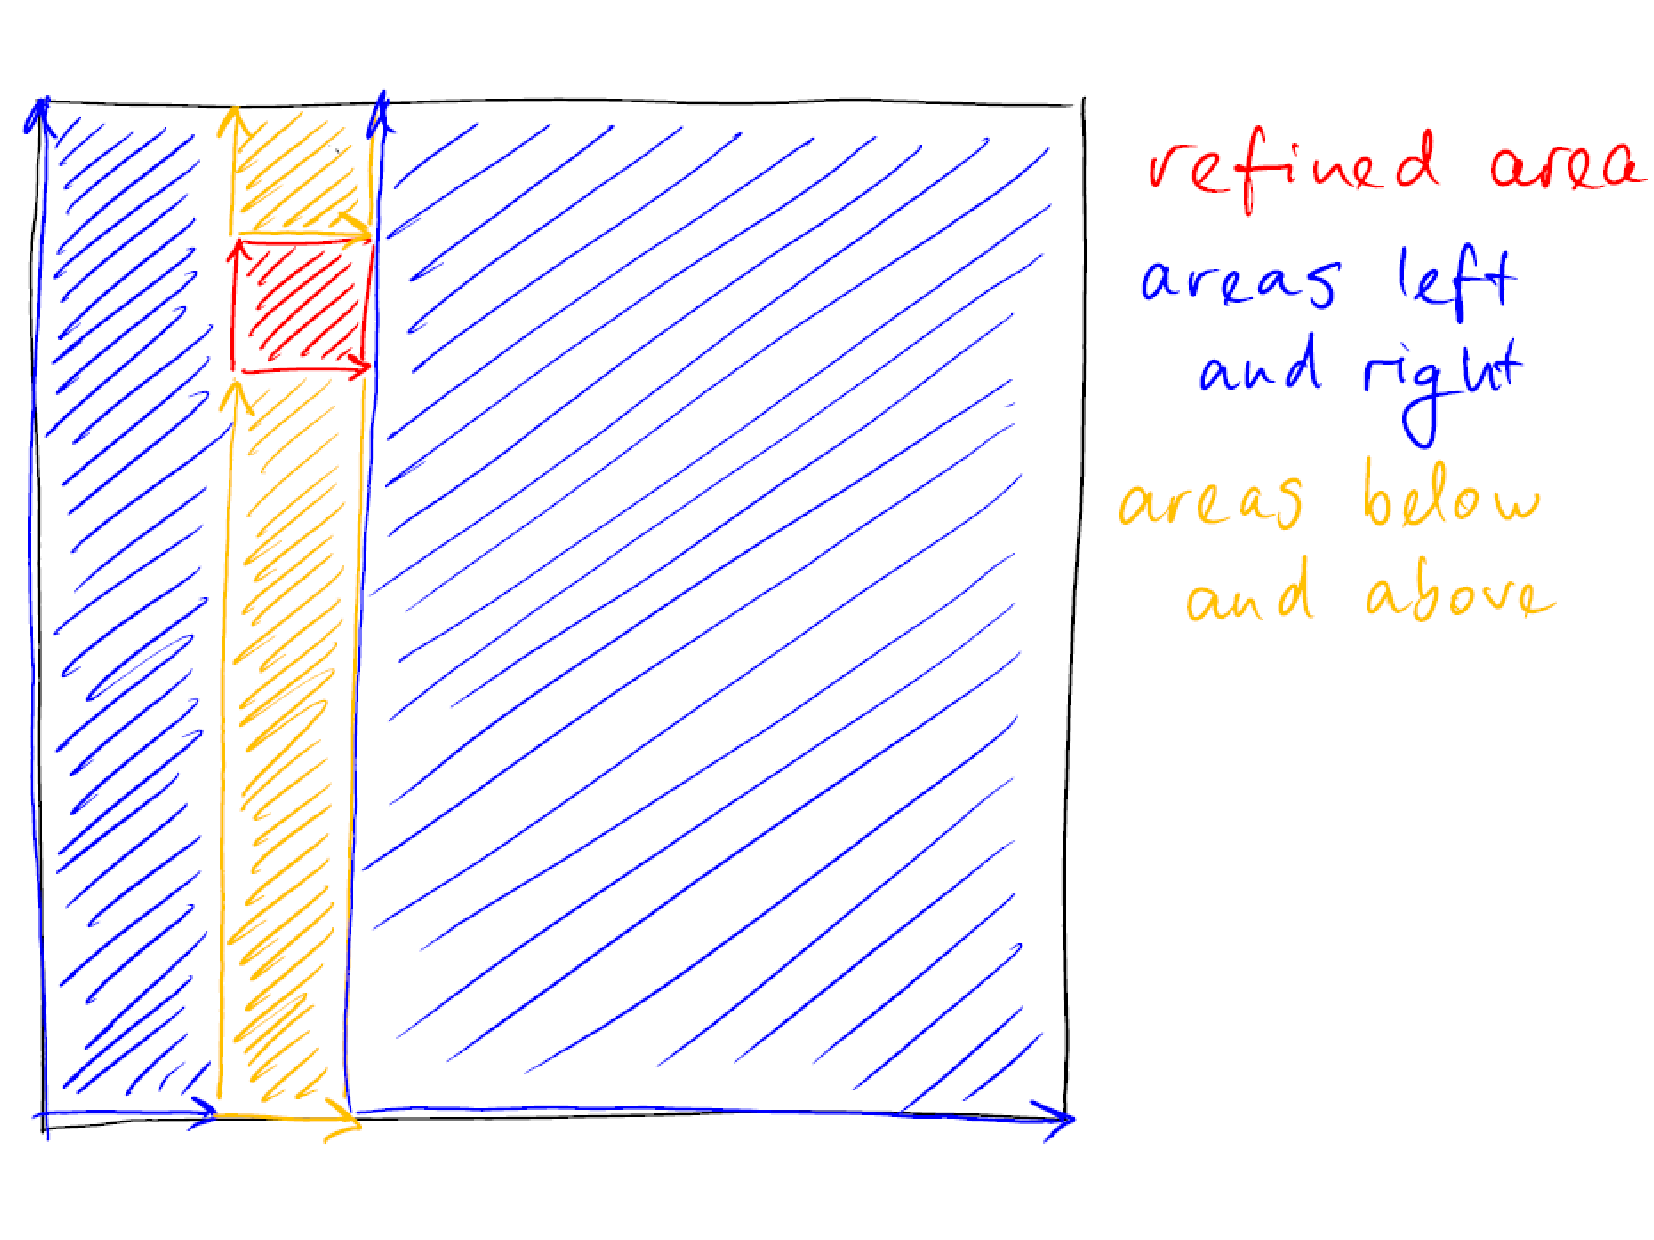
\includegraphics[width=.8\textwidth]{schematics.pdf}
 \end{figure}
\end{frame}
%---------------------------------------------------------------------
\begin{frame}
 \frametitle{Results - Level 3 with refinement}
 \begin{figure}[H]
  \centering
  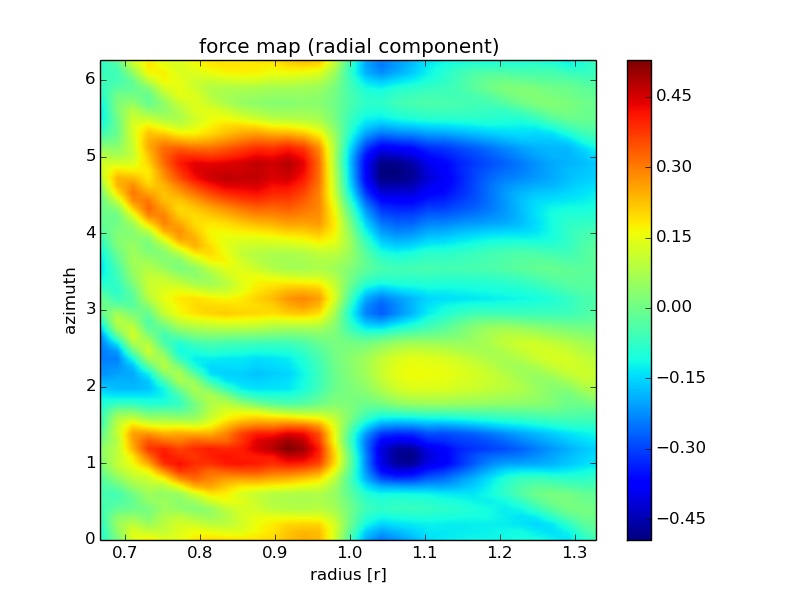
\includegraphics[width=.5\textwidth]{radial_refined_lvl3.png} 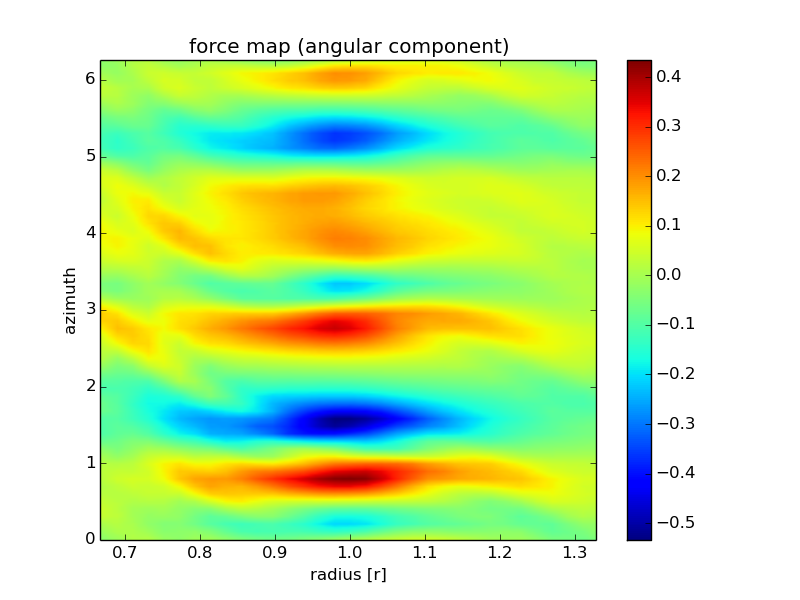
\includegraphics[width=.5\textwidth]{angular_refined_lvl3.png}
 \end{figure} 
\end{frame}
%---------------------------------------------------------------------
\begin{frame}
 \frametitle{Differences to Level 0 - radial component}
 \begin{figure}[H]
  \centering
  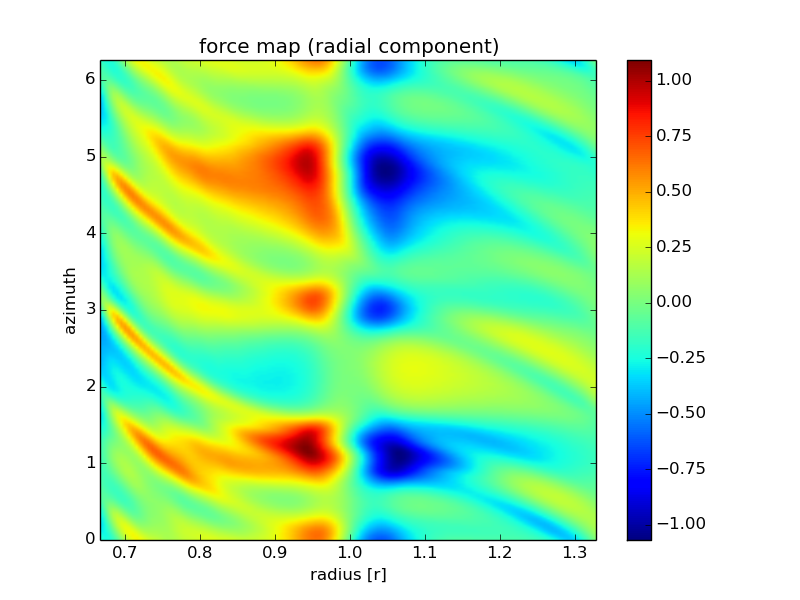
\includegraphics[width=.4\textwidth]{radial_force.png} 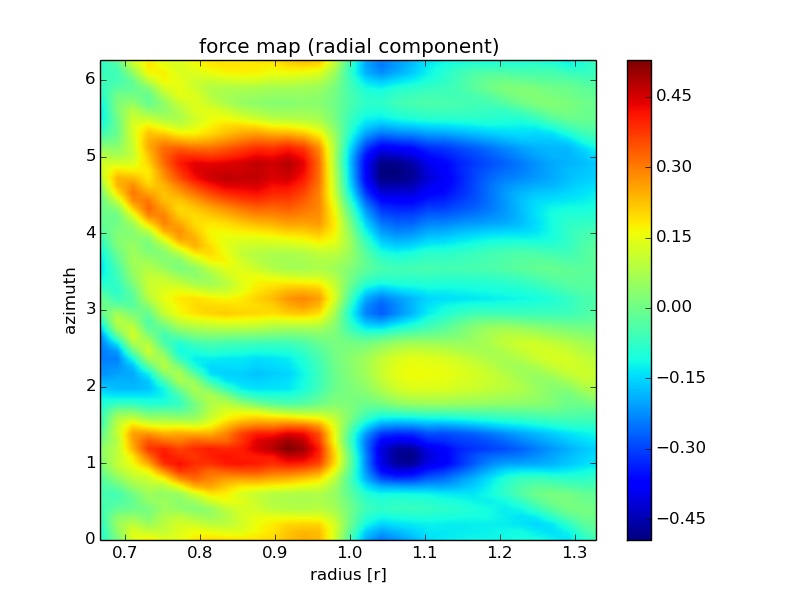
\includegraphics[width=.4\textwidth]{radial_refined_lvl3.png} \\
  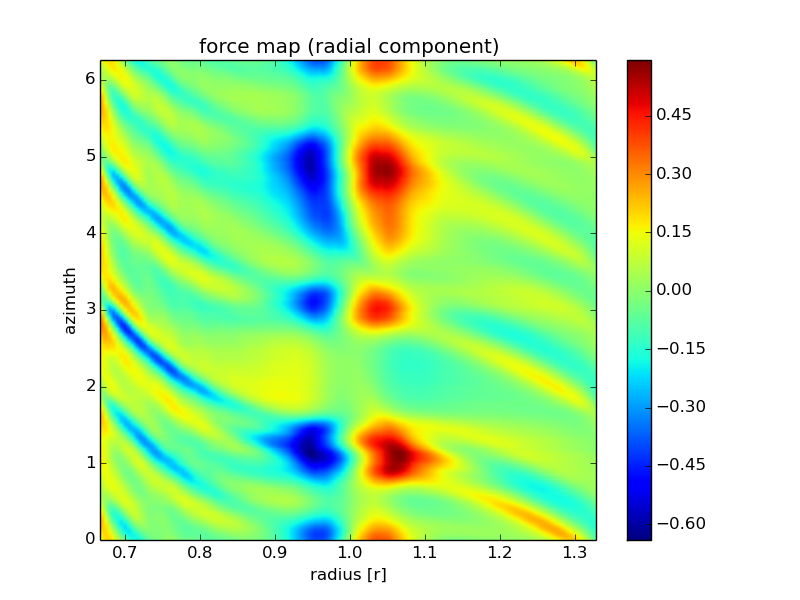
\includegraphics[width=.4\textwidth]{radial_refined_diff3.png}
 \end{figure} 
\end{frame}
%---------------------------------------------------------------------
\begin{frame}
 \frametitle{Differences to Level 0 - angular component}
 \begin{figure}[H]
  \centering
  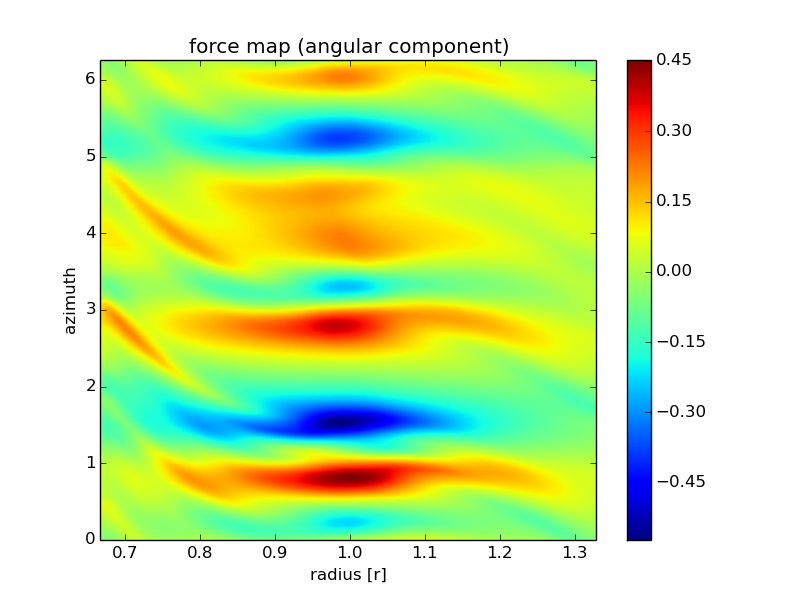
\includegraphics[width=.4\textwidth]{angular_force.png} 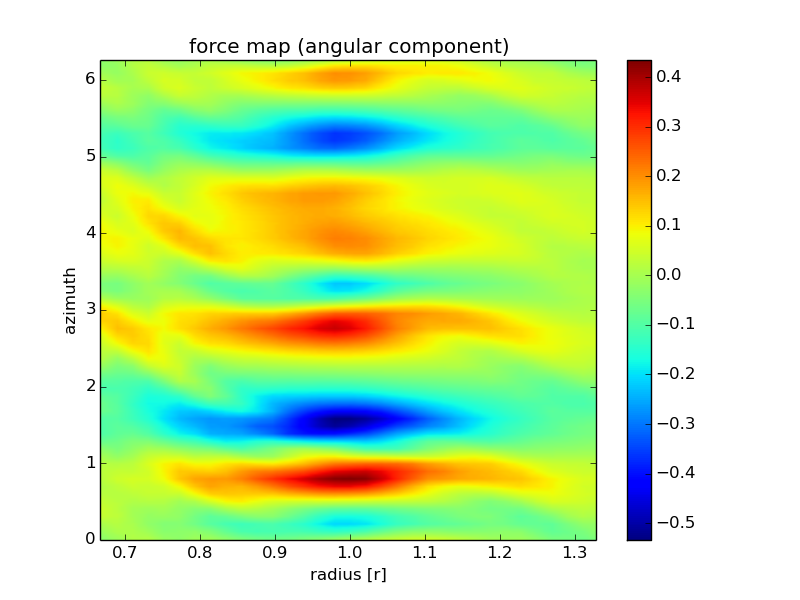
\includegraphics[width=.4\textwidth]{angular_refined_lvl3.png} \\
  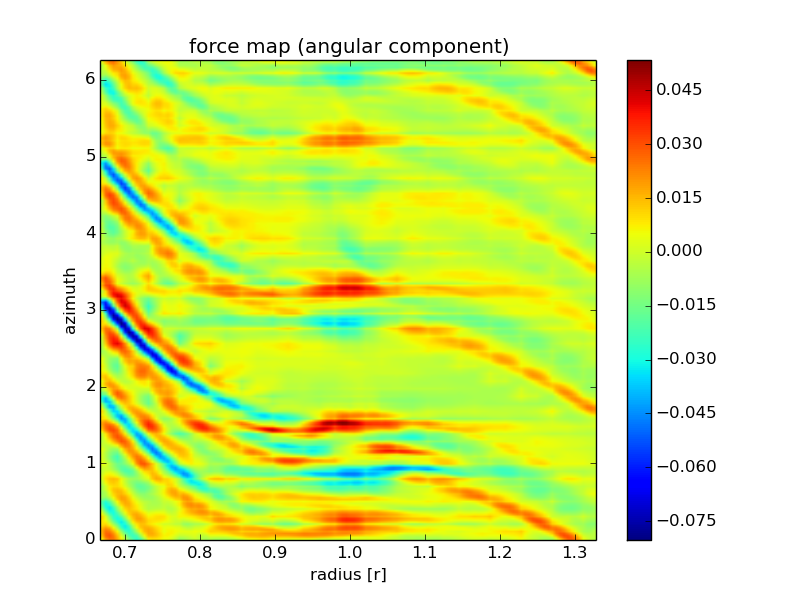
\includegraphics[width=.4\textwidth]{angular_refined_diff3.png}
 \end{figure} 
\end{frame}
%---------------------------------------------------------------------
\begin{frame}
 \frametitle{Maximal difference in a row}
 \begin{figure}[H]
  \centering
  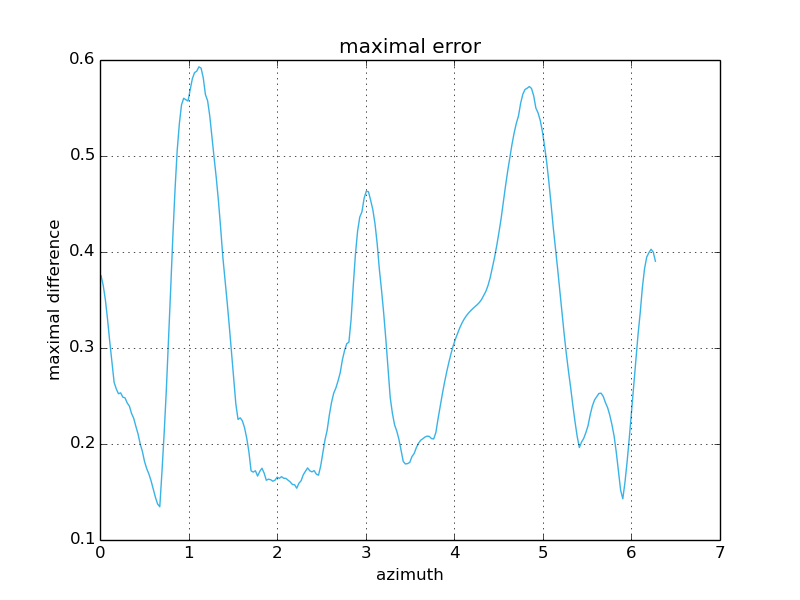
\includegraphics[width=.4\textwidth]{radial_refined_error3.png} 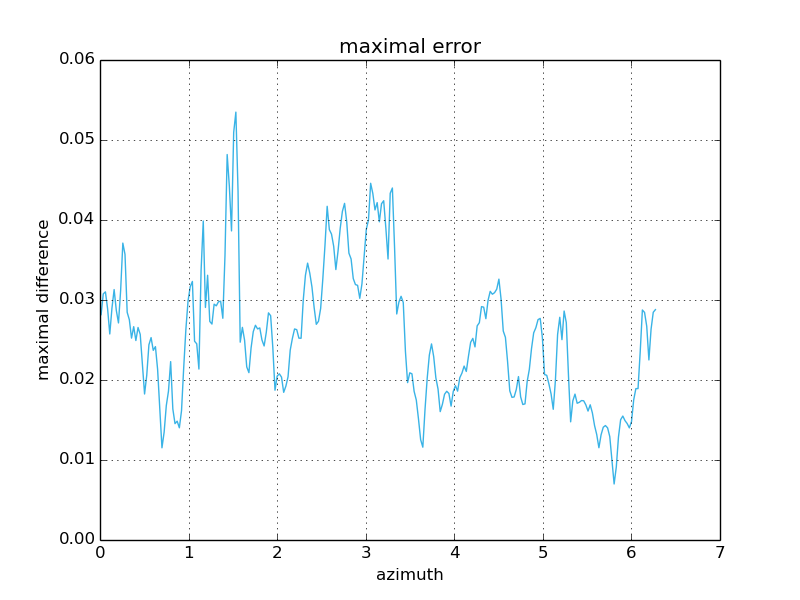
\includegraphics[width=.4\textwidth]{angular_refined_error3.png} \\
  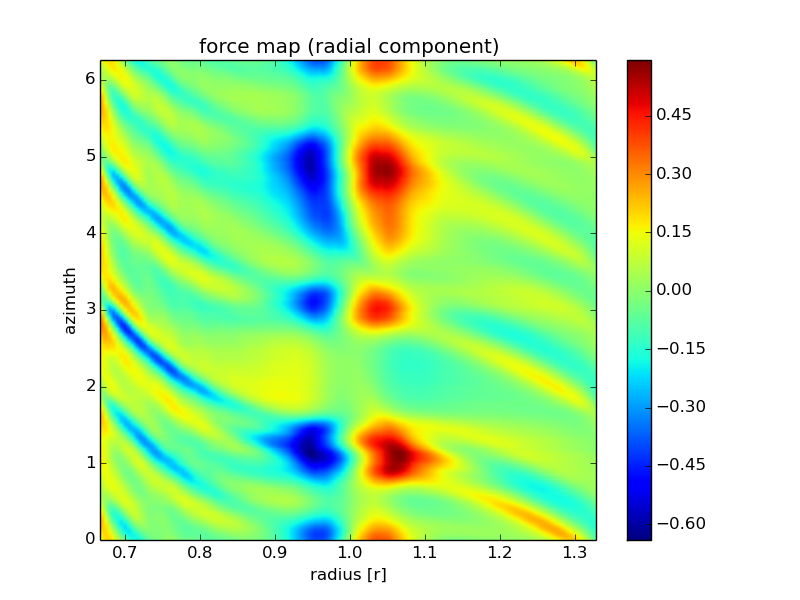
\includegraphics[width=.4\textwidth]{radial_refined_diff3.png} 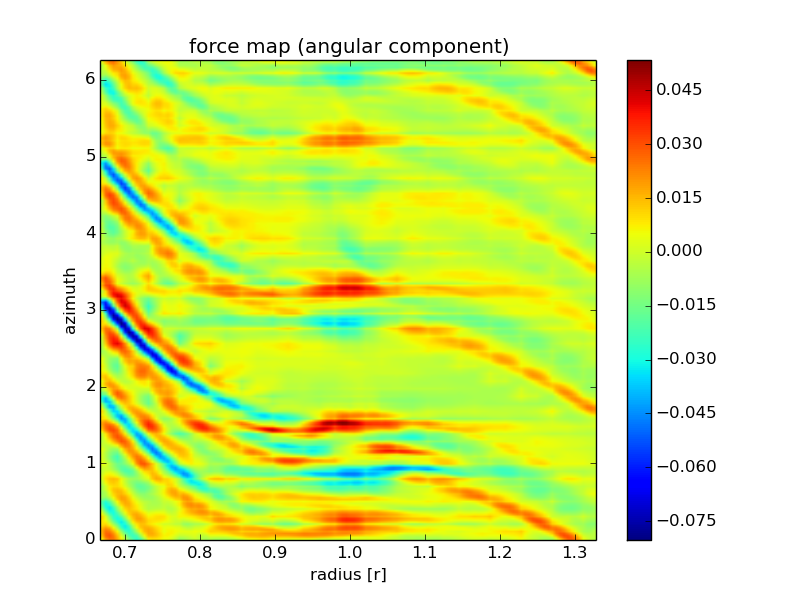
\includegraphics[width=.4\textwidth]{angular_refined_diff3.png}
\end{figure}
\end{frame}
%---------------------------------------------------------------------
\begin{frame}
 \frametitle{Improvement by refinement - radial component}
 \begin{figure}[H]
  \centering
  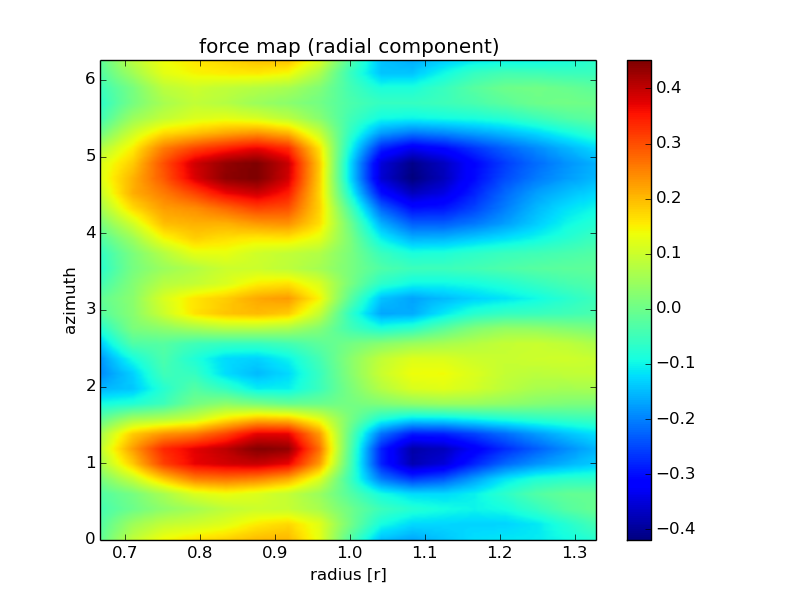
\includegraphics[width=.4\textwidth]{radial_pure_lvl3.png} 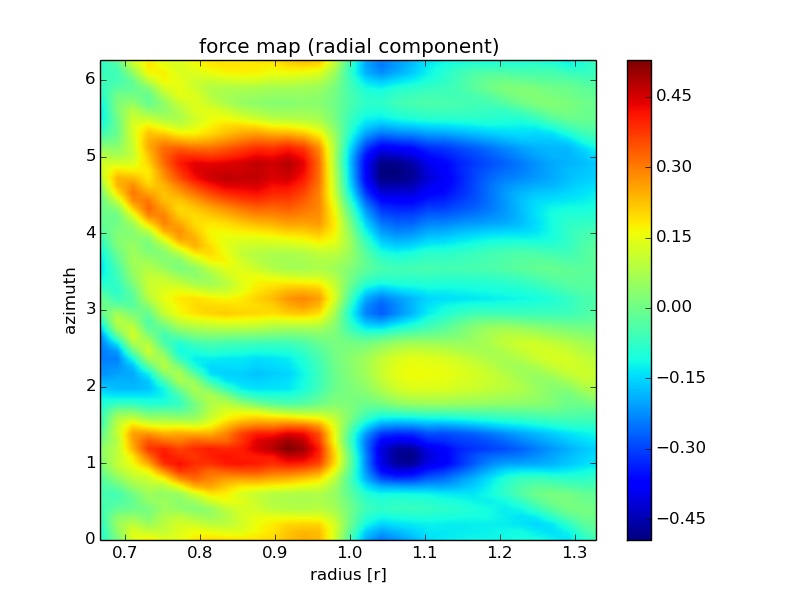
\includegraphics[width=.4\textwidth]{radial_refined_lvl3.png} \\
  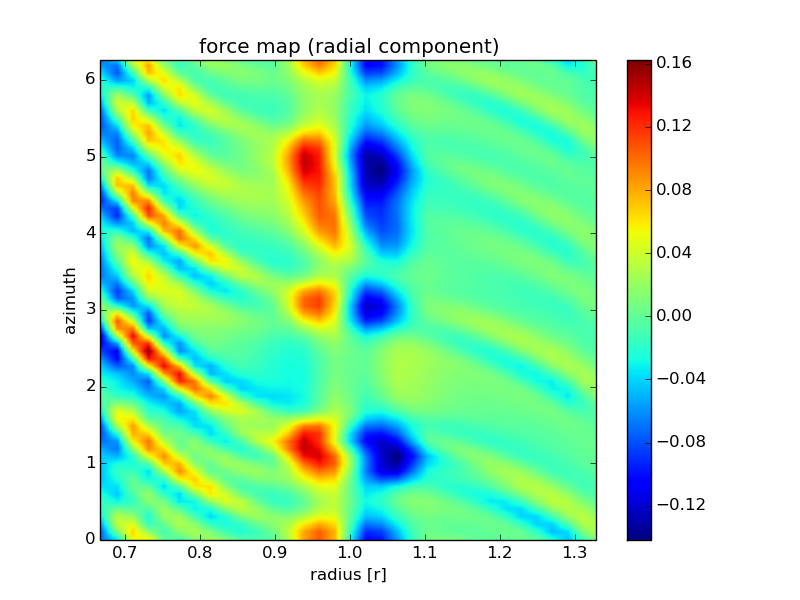
\includegraphics[width=.4\textwidth]{radial_puretorefined_diff3.png}
\end{figure}
\end{frame}
%---------------------------------------------------------------------
\begin{frame}
 \frametitle{Comparison to Level 2 - angular component}
 \begin{figure}[H]
  \centering
  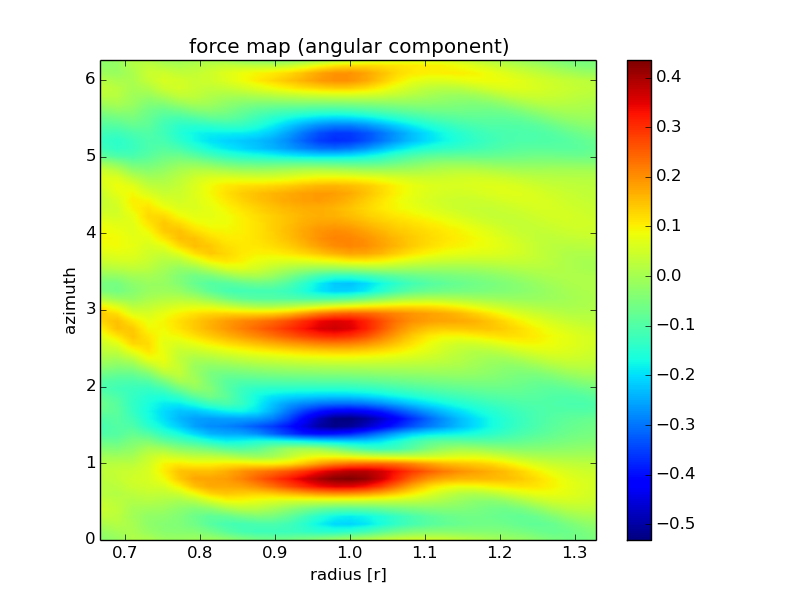
\includegraphics[width=.4\textwidth]{angular_pure_lvl2.png} 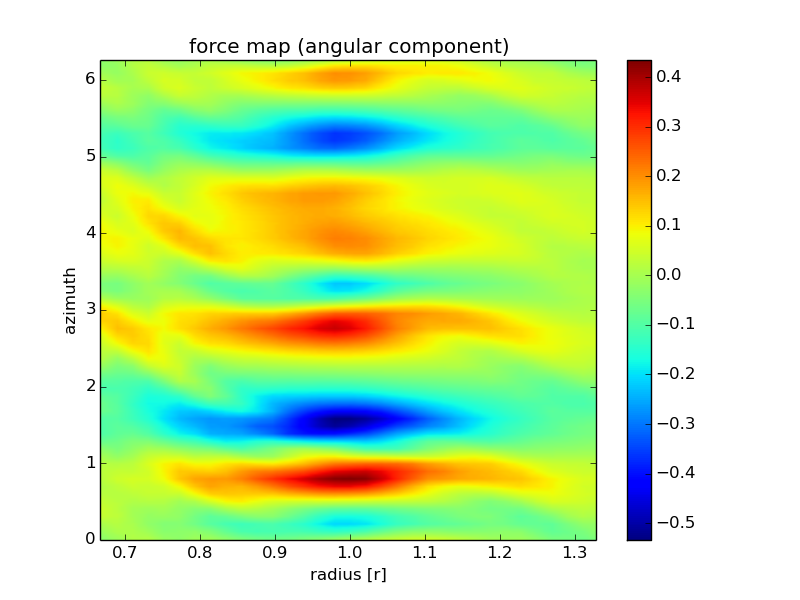
\includegraphics[width=.4\textwidth]{angular_refined_lvl3.png} \\
  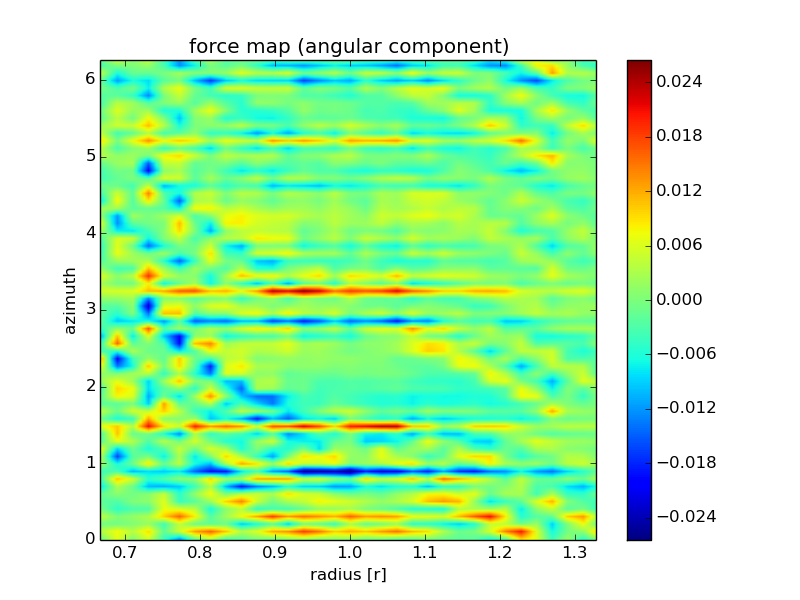
\includegraphics[width=.4\textwidth]{angular_puretorefined_diff2to3.png}
\end{figure}
\end{frame}
%---------------------------------------------------------------------

\begin{frame}
 \frametitle{How can we improve this?}
\begin{itemize}
  \item Let's look at another strategy with an \textbf{adaptive lookup}
  \begin{itemize}
  \item Increase level range [0,5]
  \item Use distance to determine lookup level
  \end{itemize}
 \end{itemize}

 \begin{figure}[H]
  \centering
  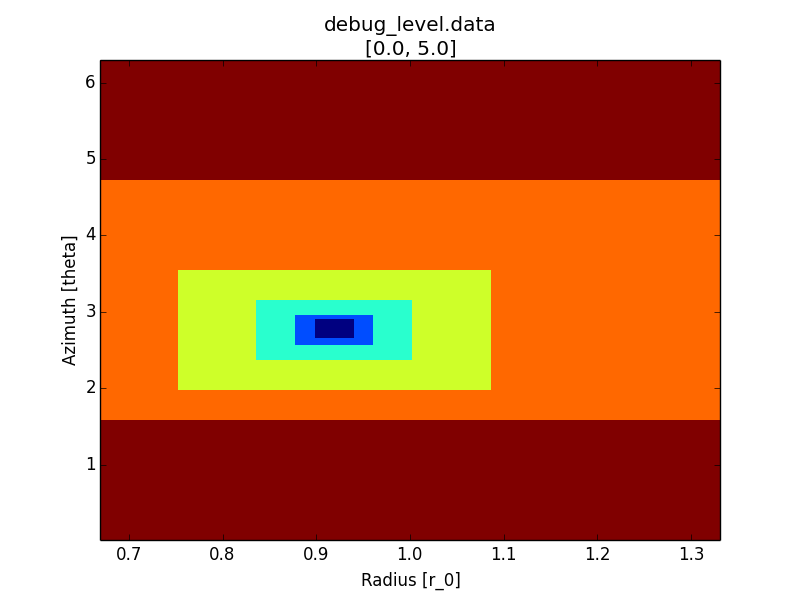
\includegraphics[width=.5\textwidth]{../../../Sara/plots/adaptive_lookup.png}     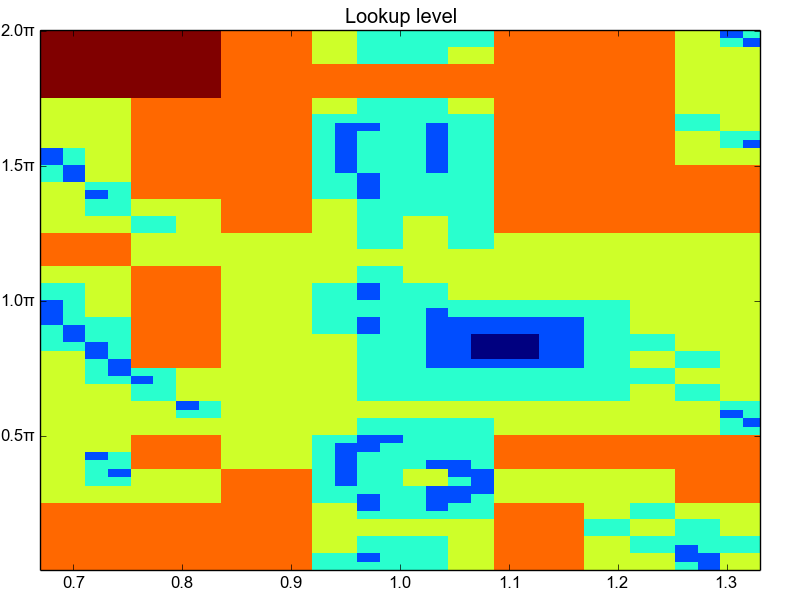
\includegraphics[width=.45\textwidth]{../../../Sara/run/default/debug_level-euclid.png}
\end{figure}
\end{frame}
%---------------------------------------------------------------------
\begin{frame}
 \frametitle{Three Optimization Steps}
  \begin{enumerate}
  
  \item Adaptive Lookup:
  \begin{itemize}
     \item[•] Increase levels with distance
  \end{itemize}
  
  \item Lookup Refinement by mass-spread:
  \begin{itemize}
     \item[•] For higher level cells, the distribution of mass at level 0 cells is an indicator for the accuracy of the higher level cells.
     \item[•] Measure "spread" as difference between max and min of level 0 masses of the cell.
     \item[•] User lower levels if cell "spread" is larger than an arbitrary predefined value.
     \item[•] This value has huge performance over accuracy implications.
  \end{itemize} 
  
  \item Centre of Mass: Correction
  \begin{itemize}
     \item[•] Centre of mass usually is not at the centre of cell
  \end{itemize}
  
  \end{enumerate}  
\end{frame}
%---------------------------------------------------------------------
\begin{frame}
 \frametitle{More about adaptive Code - Centre of Mass Correction}
\begin{itemize}
  \item A cell's centre of mass can vary wildly as the levels increase
 \end{itemize}
 \begin{figure}[H]
  \centering
  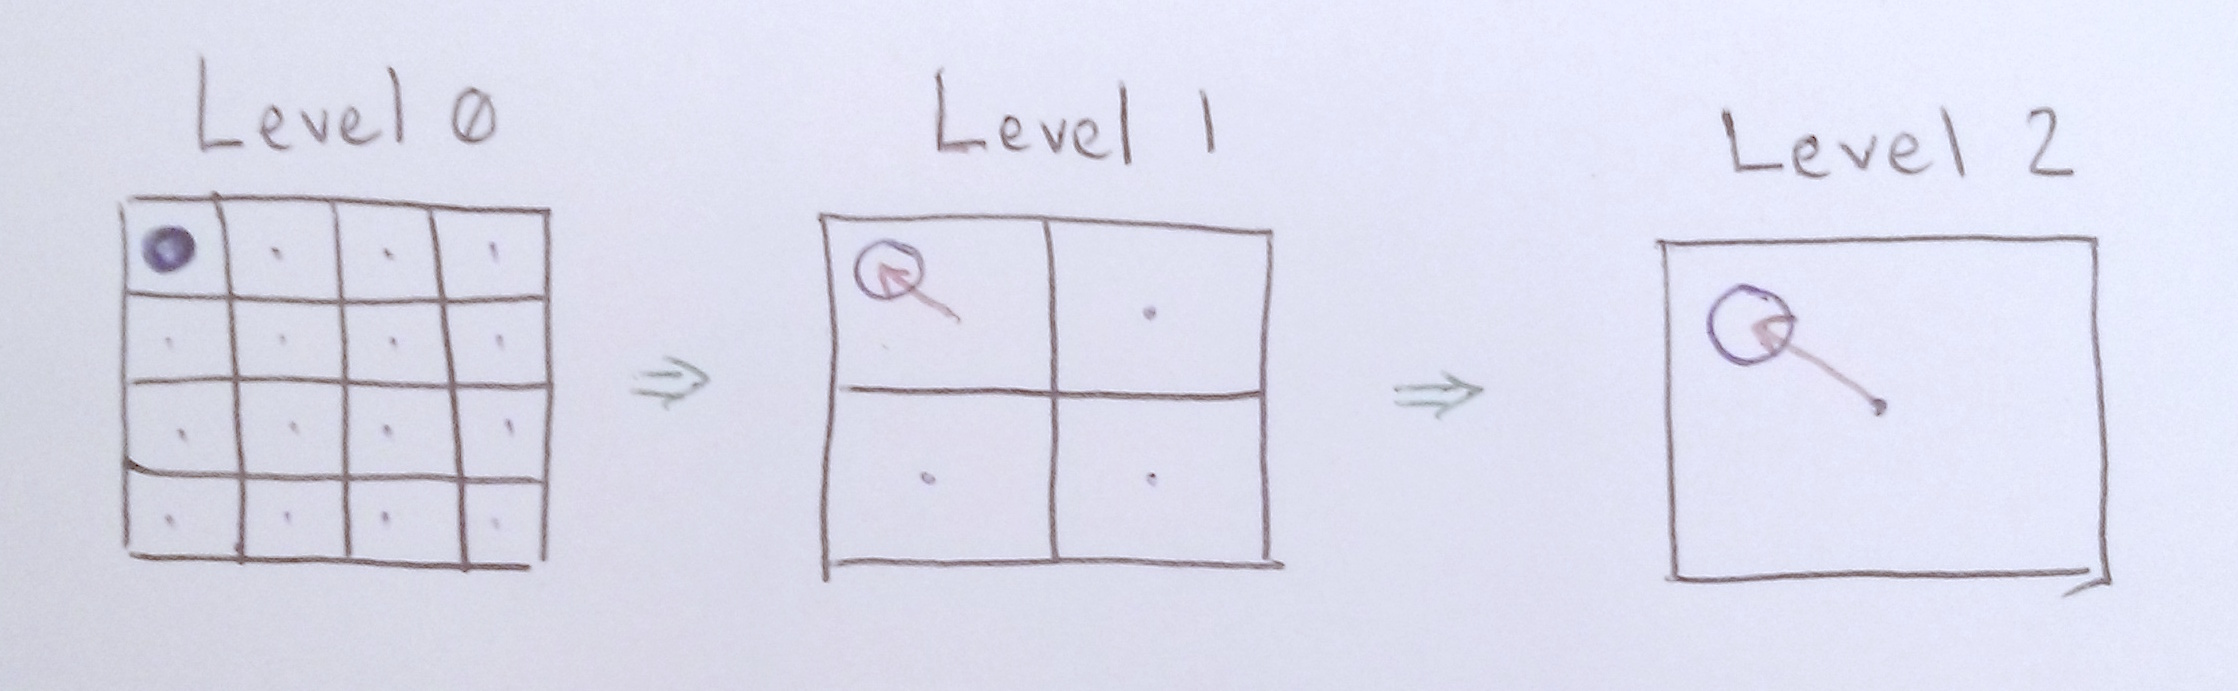
\includegraphics[width=.7\textwidth]{../../../Sara/plots/COM_correction.png}     
\end{figure}
\end{frame}
%---------------------------------------------------------------------
\begin{frame}
 \frametitle{More about adaptive Code - Centre of Mass Correction}
\begin{itemize}
  \item Correcting for the centre of mass
 \end{itemize}
 \begin{figure}[H]
  \centering
  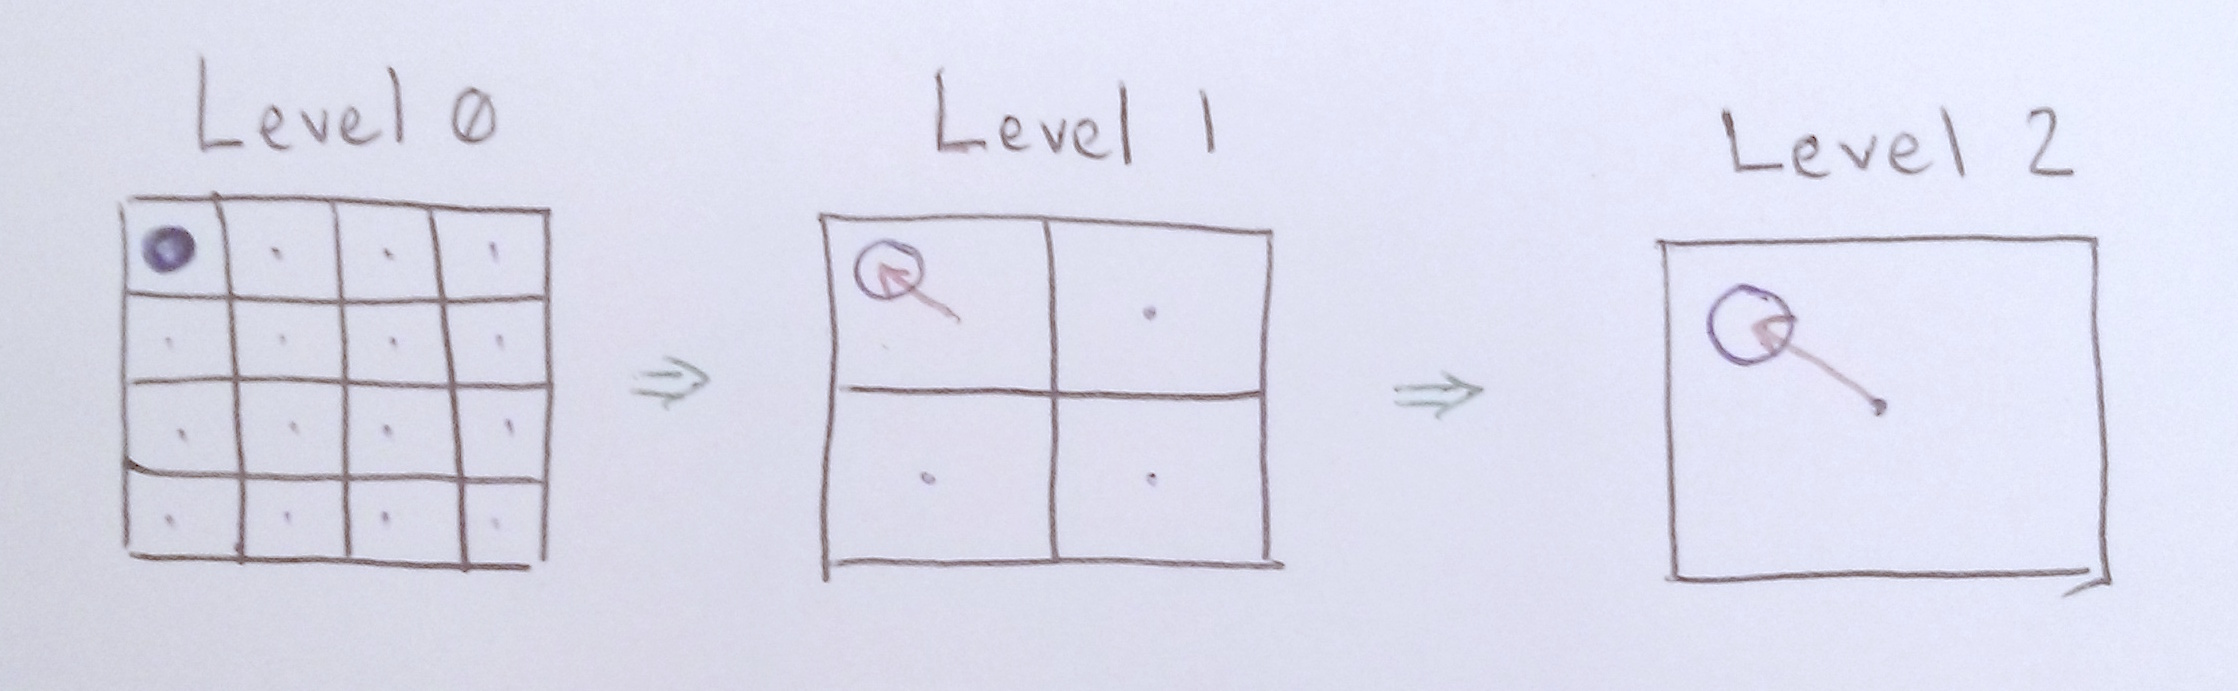
\includegraphics[width=.7\textwidth]{../../../Sara/plots/COM_correction.png}     
\end{figure}
\begin{itemize}
  \item Improvement: error reduction from 1.8\% $\rightarrow$ 1.4\% in the radial component

 \end{itemize}
\end{frame}
%---------------------------------------------------------------------
\begin{frame}
 \frametitle{More about adaptive Code - Centre of Mass Correction}
\begin{itemize}
  \item Correcting for the centre of mass
 \end{itemize}
 \begin{figure}[H]
  \centering
  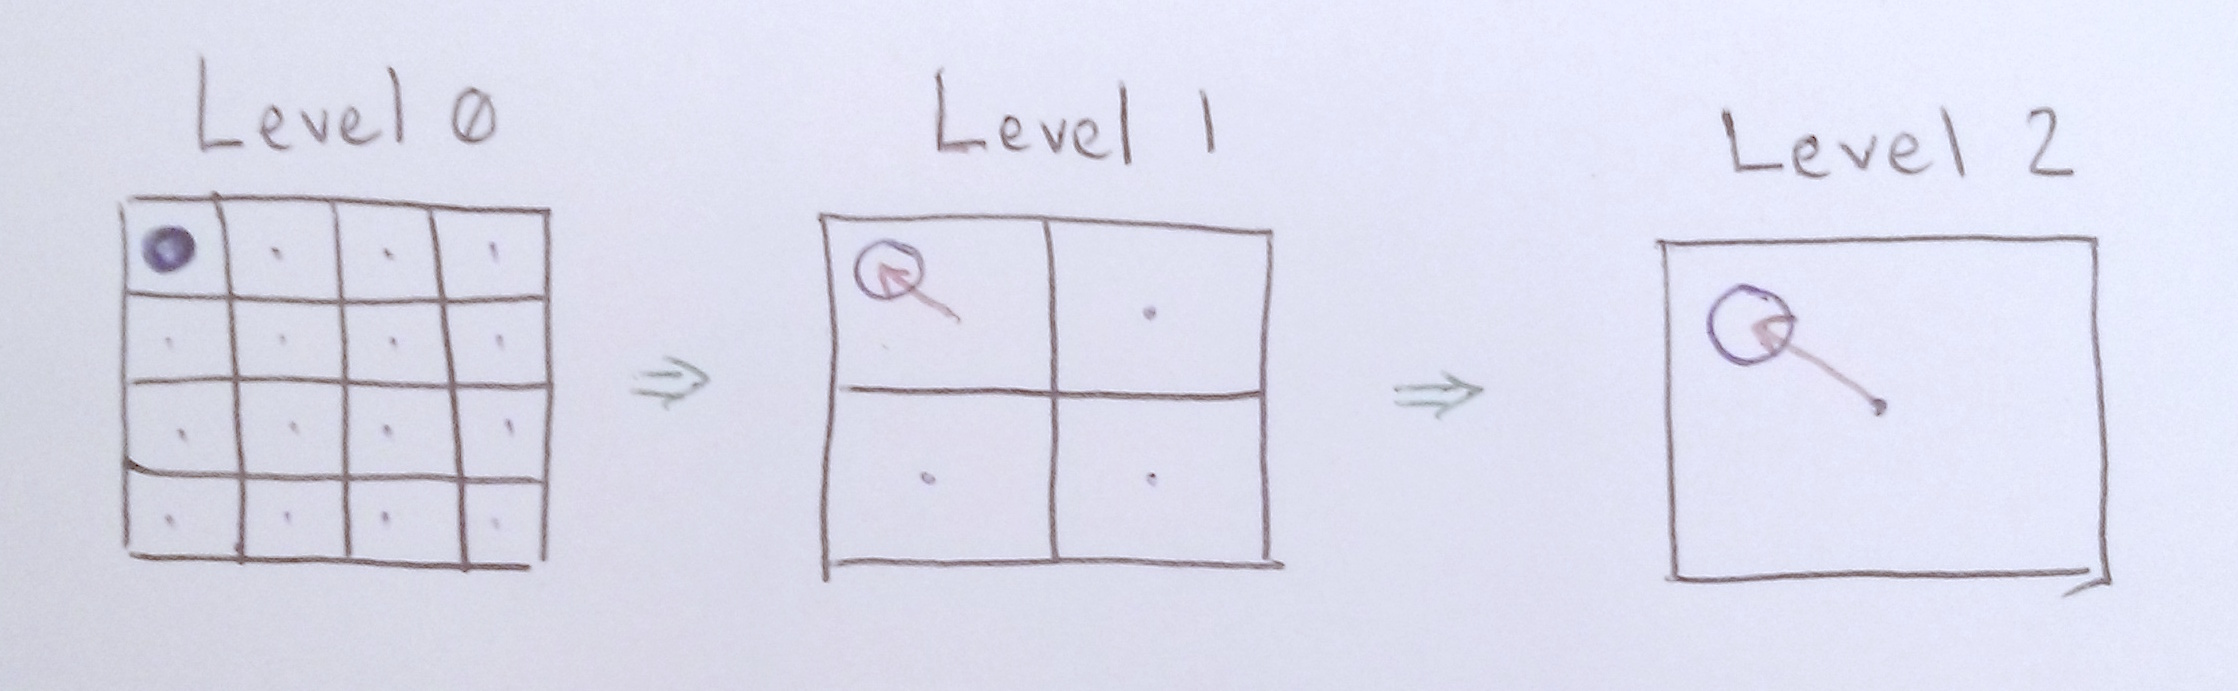
\includegraphics[width=.7\textwidth]{../../../Sara/plots/COM_correction.png}     
\end{figure}
\begin{itemize}
  \item Improvement: error reduction from 1.8\% $\rightarrow$ 1.4\% in the radial component
  \item Further Work: Carthesian math is an approximation, should work better in polar coordinates?
 \end{itemize}
\end{frame}
%---------------------------------------------------------------------

%---------------------------------------------------------------------
\begin{frame}
 \frametitle{Result}
\begin{itemize}
  \item Simulation time: Level 0: 11s, Level 5-0: 4s
  \item Error bound: \textless 2\% at peaks
  \item Oscillation patterns still exist
 \end{itemize}

 \begin{figure}[H]
  \centering
  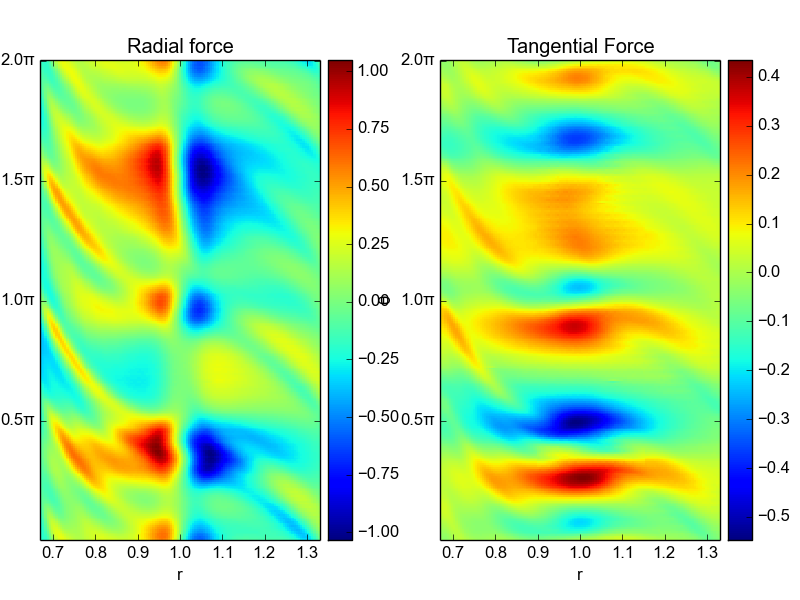
\includegraphics[width=.5\textwidth]{../../../Sara/run/default/forcesA-euclid.png}     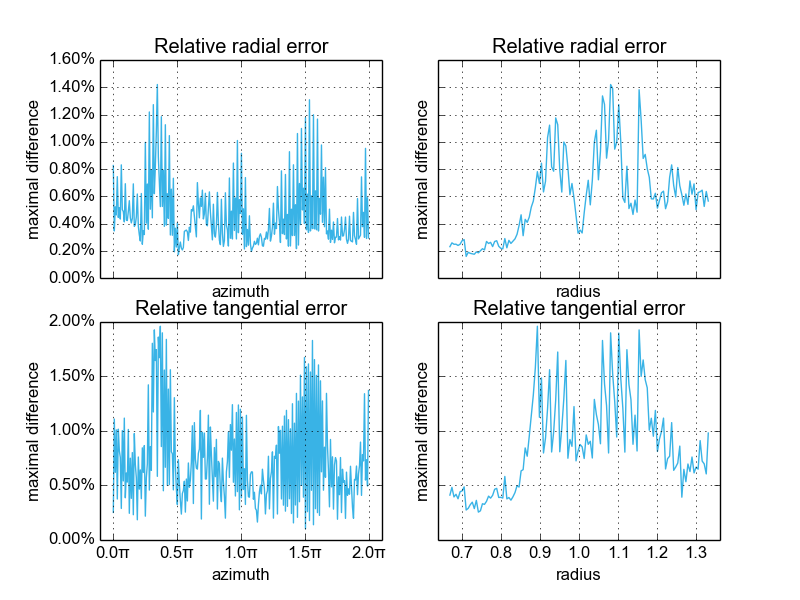
\includegraphics[width=.5\textwidth]{../../../Sara/run/default/diff_1D.png}
\end{figure}
\end{frame}

%---------------------------------------------------------------------
\begin{frame}
 \frametitle{Results - Relative Diff with Level 0 vs. Adaptive}
\begin{itemize}
  \item MSE is quite small
  \begin{itemize}
    \item Large areas have almost no error
  \end{itemize}
  \item Problem: Oscillations still exist
  \item Huge error spike in COM correction (lower MSE @ 0.000012)
 \end{itemize}

 \begin{figure}[H]
  \centering
  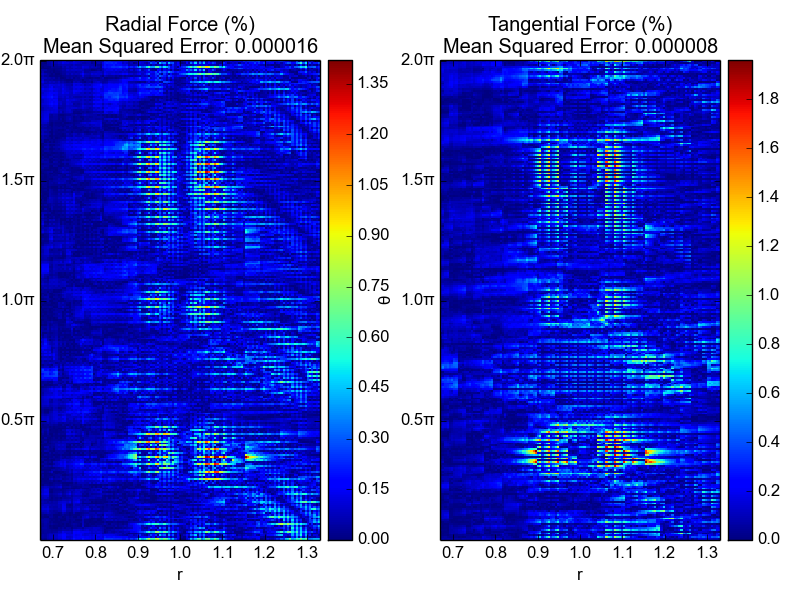
\includegraphics[width=.7\textwidth]{../../../Sara/run/default/diff_2D-euclid.png} 

\end{figure}
\end{frame}
%---------------------------------------------------------------------



\begin{frame}
 \frametitle{Future Work with Adaptive Approach}


	\begin{itemize}
  		\item Address oscillations
  		\begin{itemize}
    			\item Bilinear interpolation with ghost cells
    			\item Overlaping adaptive higher levels
  		\end{itemize}
  		\item Address centre of mass correction errors
  		\begin{itemize}
    			\item Address spikes (not just by increasing epsilon )
    			\item Polar-corrected approximation of centre of mass
  		\end{itemize}
	\end{itemize}





 \begin{figure}[H]
  \centering
  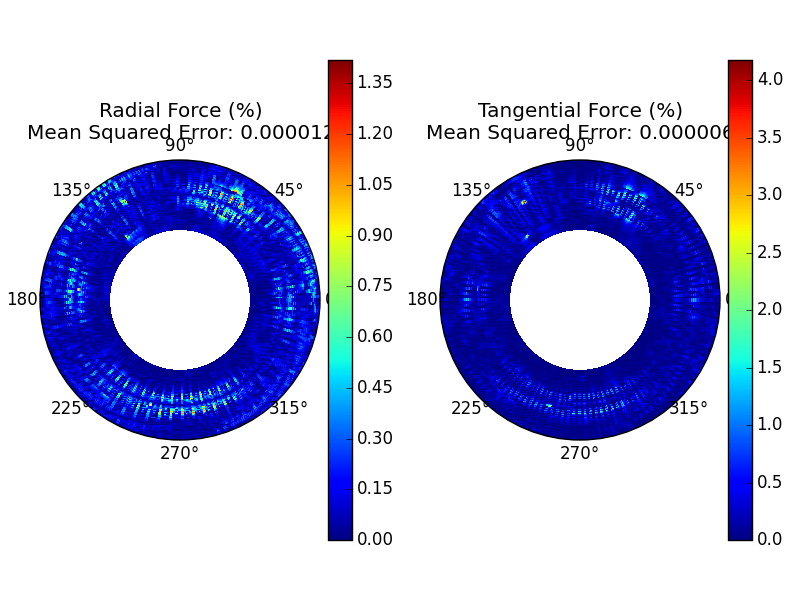
\includegraphics[width=.5\textwidth]{../../../Sara/run/default/diff_2D-polar.png} 

 \end{figure}
  
\end{frame}
%---------------------------------------------------------------------

\begin{frame}
 \frametitle{Thanks for listening!}
 \begin{center}
  Questions?
 \end{center}
\end{frame}
%---------------------------------------------------------------------
% Supplementary slides
% if there's enough time or we need to fill time...
%---------------------------------------------------------------------
\begin{frame}
 \frametitle{Results for Level 1 with refinement}
 \begin{figure}[H]
  \centering
  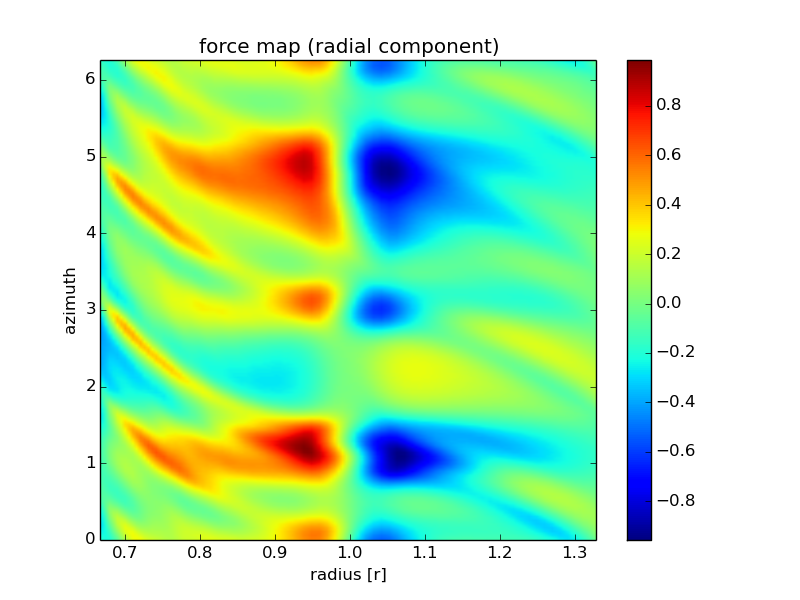
\includegraphics[width=.3\textwidth]{radial_refined_lvl1.png} 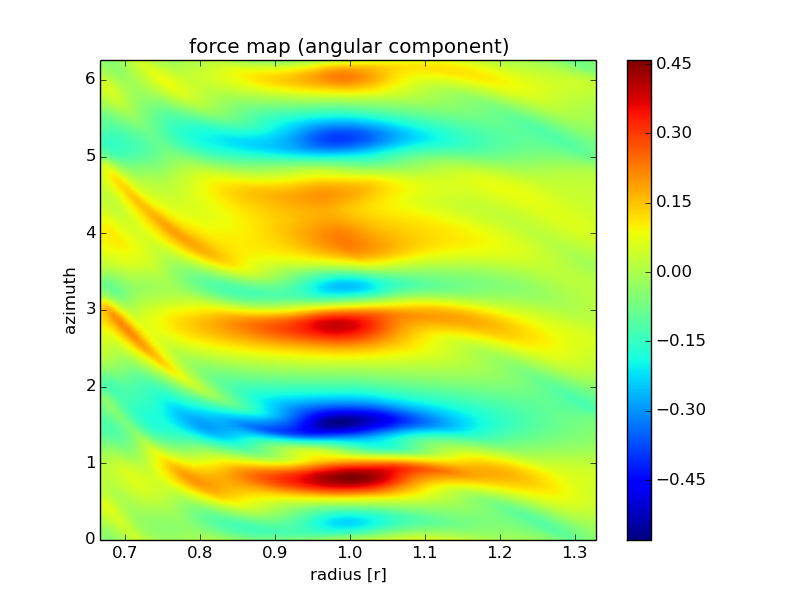
\includegraphics[width=.3\textwidth]{angular_refined_lvl1.png} \\
  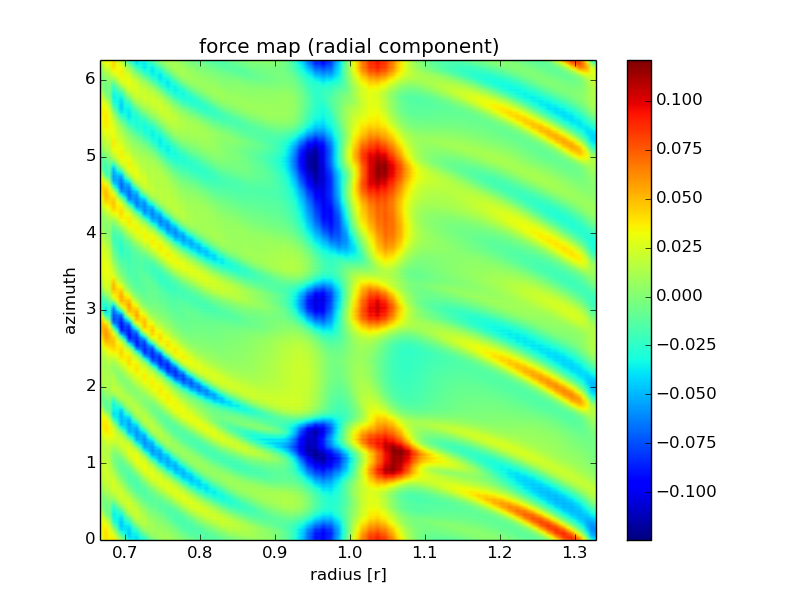
\includegraphics[width=.3\textwidth]{radial_refined_diff1.png} 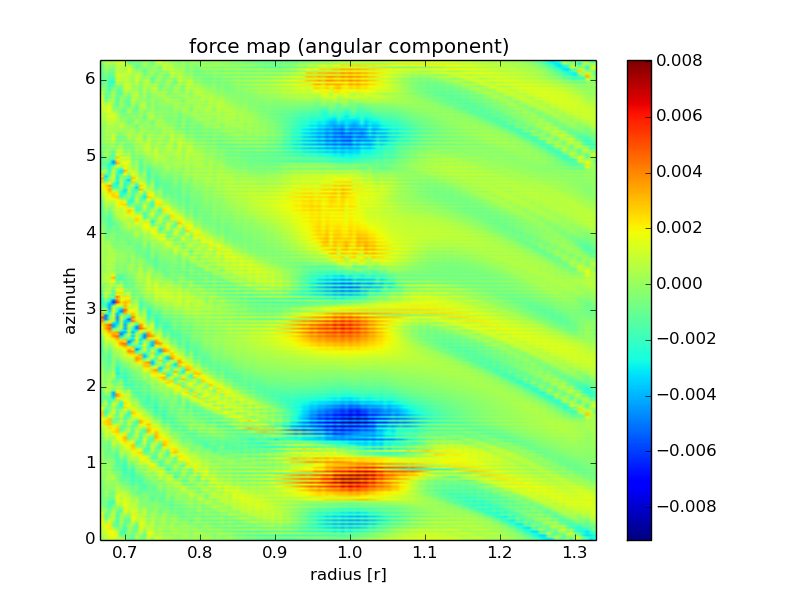
\includegraphics[width=.3\textwidth]{angular_refined_diff1.png} \\
  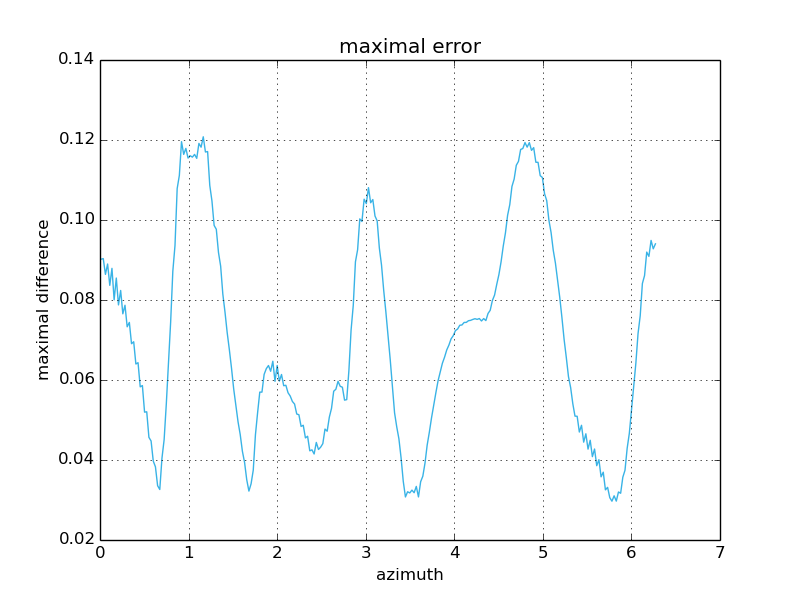
\includegraphics[width=.3\textwidth]{radial_refined_error1.png} 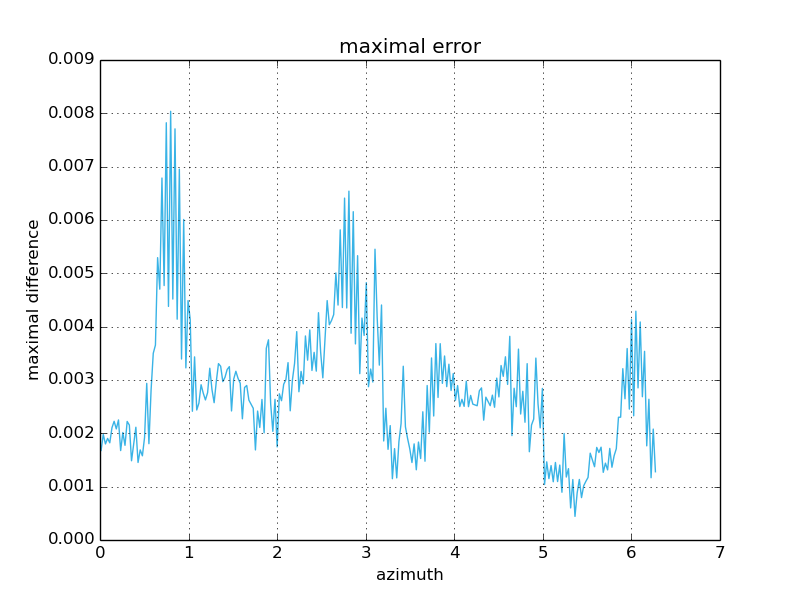
\includegraphics[width=.3\textwidth]{angular_refined_error1.png} 
\end{figure}
\end{frame}
%---------------------------------------------------------------------
\begin{frame}
 \frametitle{InvSqrt}
 \url{http://en.wikipedia.org/wiki/Fast_inverse_square_root}
\end{frame}
%---------------------------------------------------------------------
\begin{frame}[fragile]
 \frametitle{Custom InvSqrt}
  \lstset{
    language=[90]Fortran,
    aboveskip=3mm,
    belowskip=3mm,
    showstringspaces=false,
    columns=fullflexible,
    basicstyle={\tiny\ttfamily},
    numbers=none,
    numberstyle=\small\color{gray},
    keywordstyle=\color{mauve},
    commentstyle=\color{dkgreen},
    stringstyle=\color{blue},
    breaklines=true,
    breakatwhitespace=false,
    tabsize=3
}
  \begin{lstlisting}
   REAL(8) FUNCTION InvSqrt (x)
    IMPLICIT NONE
    TYPE casting
        REAL(8) :: x
    END TYPE casting
    REAL(8), INTENT(in) :: x
    ! casting
    TYPE(casting), TARGET :: pointerTo
    ! Encode data as an array of integers
    INTEGER(8), DIMENSION(:), ALLOCATABLE :: enc
    INTEGER(8) :: length
    INTEGER(8) :: magic_number = 6910469410427058089
    REAL(8) :: xhalf
    xhalf = .5*x
    ! transfer to heap
    pointerTo%x = x
    ! encode a memory section from a type to other
    length = size(transfer(pointerTo, enc))
    allocate(enc(length))
    ! encoded to integer
    enc = transfer(pointerTo, enc)  ! evil floating point bit level hacking
    enc(1) = magic_number - rshift(enc(1),1)  ! wtf! (for int64: 0x5fe6eb50c7b537a9 = 6910469410427058089)
    ! decode
    pointerTo = transfer(enc, pointerTo)
    ! dealloc
    deallocate(enc)

    InvSqrt = pointerTo%x*(1.5 - xhalf*pointerTo%x*pointerTo%x)
END FUNCTION InvSqrt
  \end{lstlisting}

\end{frame}
%---------------------------------------------------------------------


\end{document}